% ======================================================================
% capitulos/linea2/e3_sistema_funcional.tex
% ----------------------------------------------------------------------
% LÍNEA CE02 — INGENIERÍA DE SOFTWARE
% S2 · E3: SISTEMA DE SOFTWARE FUNCIONAL INTEGRADO (alineado con CE023)
% Fuente: repositorio cristian-csc/Wisp-ISP, rama main, commit 98d64db (19/11/2026)
% Diagramas: diagramas/ce02_e3/*.mmd (Mermaid, editables en Lucidchart/draw.io),
%            renderizados en imagenes/linea2/d0*.png
% Catálogo de endpoints: tools/extraer_endpoints.py + tools/catalogo_api.py
% ======================================================================
\chapter{Sistema de Software Funcional Integrado}
\label{chap:ce02-e3}

\entregable{CE02 --- Ingeniería de Software · competencia CE023 Programación}
{Semestre 2 · Entregable 3: Sistema de Software Funcional Integrado}
{CE0233 Sistema web integrado con base de datos · CE0234 Aplicación full-stack desplegable · CE0236 Aplicación móvil integrada con servicios digitales}
{Sistema en producción en \texttt{https://wispfibra.com}. Incluye capturas de las pantallas internas del panel con datos anonimizados; pendientes las de la app móvil.}

\begin{table}[H]
\centering
\caption{Datos del sistema entregado.}
\label{tab:ce02-e3-ficha}
\small
\begin{tabularx}{\textwidth}{L{3.6cm}X}
\toprule
Sistema & WISP Control --- Sistema de Gestión Integral para ISP de Fibra Óptica Multi-Zona \\
Despliegue & \texttt{https://wispfibra.com} (sitio), \texttt{/app} (panel), \texttt{/api} (API, usada por la app móvil) \\
Repositorio & \texttt{https://github.com/cristian-csc/Wisp-ISP} \\
Versión documentada & Rama \texttt{main}, commit \texttt{98d64db} (19/11/2026); 86 commits desde el 19/10/2026 \\
App móvil & Expo SDK 54, paquete \texttt{com.wispfibra.app} \\
\bottomrule
\end{tabularx}
\end{table}

\section*{Resumen ejecutivo}
\addcontentsline{toc}{section}{Resumen ejecutivo}

El sistema resuelve el problema central de WISP: llevar a una sola plataforma lo que antes
se hacía en papel, en WhatsApp y entrando a mano a 13 routers. Cubre el ciclo de vida
completo del cliente ---captación en campo, aprobación, instalación con registro de caja,
borne y ONU, cobranza, corte automático por mora, reactivación al pagar, averías y retiro
del equipo--- y los procesos que lo sostienen: planta externa, inventario de ONU, red de
zonas con WireGuard, finanzas, comunicación por WhatsApp y seguimiento de vendedores.

Se usa de tres formas. El \textbf{personal de oficina} (administración y atención al
cliente) trabaja en el panel web \texttt{wispfibra.com/app}. El \textbf{personal de campo}
(técnicos y vendedores) y los \textbf{clientes} usan una app móvil que muestra a cada rol
solo sus módulos. El \textbf{público} consulta planes y cobertura en el sitio
\texttt{wispfibra.com}. Todos consumen la misma API REST: 169 endpoints en 19 módulos,
protegidos por JWT, tipo de cuenta y módulos asignados al rol.

El sistema está desplegado en producción con Docker Compose en el servidor de la oficina y
se publica por un túnel de Cloudflare, sin abrir puertos de entrada. Este capítulo documenta
la arquitectura e integración, los flujos del negocio implementados (con diagramas editables
en Lucidchart), el código y su diseño técnico, el despliegue y el catálogo completo de la
API.

% ======================================================================
\section{Sección 1: Arquitectura e integración}
\label{sec:ce02-e3-arq}

\subsection{Arquitectura general}

La arquitectura se documentó en el entregable de requerimientos y diseño: vistas C4 de
contexto, contenedores y componentes (\cref{fig:ce02-contexto,fig:ce02-componentes,fig:ce02-c3})
y despliegue (\cref{fig:ce02-despliegue}). Es un monolito modular cliente-servidor: un
backend único organizado por dominios expone una API REST que consumen tres clientes.

\begin{table}[H]
\centering
\caption{Componentes del sistema y tamaño del código fuente (rama \texttt{main}, 19/11/2026).}
\label{tab:ce02-e3-componentes}
\small
\begin{tabularx}{\textwidth}{L{3cm}L{4cm}XL{2.6cm}}
\toprule
\textbf{Componente} & \textbf{Tecnología} & \textbf{Responsabilidad} & \textbf{Código} \\
\midrule
API REST & Python, FastAPI, SQLAlchemy 2, Pydantic 2 & 19 routers por dominio, seguridad, planificador, integración con routers y VPS & 32 archivos, 11\,636 líneas \\
Migraciones & Alembic & Esquema versionado de la base de datos & 35 migraciones, 1\,963 líneas \\
Pruebas & pytest & Pruebas de pagos y gastos & 3 archivos, 613 líneas \\
Panel web & React 19, Vite 7, TypeScript, Tailwind CSS & Administración, atención al cliente, finanzas, red & 123 archivos, 23\,692 líneas \\
App móvil & Expo SDK 54, React Native 0.81, TypeScript & Técnico, vendedor de campo y cliente & 52 archivos, 9\,067 líneas \\
Servicio WhatsApp & Node.js 20, Baileys, Express & Envío de mensajes y vinculación por QR & 1 archivo, 278 líneas \\
Sitio público & HTML, CSS, JavaScript & Planes, cobertura y contacto & 3 archivos, 2\,168 líneas \\
\bottomrule
\end{tabularx}
\end{table}

\subsection{Integración con la base de datos}

El backend accede a PostgreSQL~15 solo a través del ORM SQLAlchemy: no hay SQL concatenado
con datos del usuario. El esquema se versiona con Alembic y el contenedor del backend aplica
las migraciones pendientes en cada arranque (\texttt{alembic upgrade head}). Desde el
entregable de plataforma de datos (\cref{chap:ce02-datos}) se agregaron tres migraciones y
cuatro tablas para el modelo de roles y módulos (\texttt{roles}, \texttt{modulos\_padre},
\texttt{modulos} y \texttt{rol\_modulo}; \cref{sec:ce02-e3-roles}): el esquema actual tiene
35 migraciones y 25 tablas.

\subsection{Integración con sistemas y servicios externos}

\begin{table}[H]
\centering
\caption{Integraciones externas implementadas.}
\label{tab:ce02-e3-integraciones}
\small
\begin{tabularx}{\textwidth}{L{2.8cm}L{3.4cm}X}
\toprule
\textbf{Sistema externo} & \textbf{Mecanismo} & \textbf{Uso en el negocio} \\
\midrule
13 routers MikroTik (RouterOS 7) & SSH con llave (paramiko) por la IP del túnel WireGuard & Crear y modificar secretos PPPoE, sincronizar perfiles de planes, cortar y reactivar (address-list), ver sesiones PPPoE en vivo, terminal restringida. \\
VPS con el hub WireGuard & SSH (\texttt{wg show}, \texttt{wg set}) & Alta y baja de peers de zona y estado de cada túnel, con caché de 120 s. \\
WhatsApp & Servicio propio (Baileys) por HTTP local con token & Recordatorios, avisos de corte, confirmaciones de pago, mensajes masivos con pausas. \\
APIs Perú & HTTPS con token guardado solo en el servidor & Autocompletar nombre por DNI o razón social por RUC, con cuota mensual controlada. \\
Cloudflare & Túnel de salida (\texttt{cloudflared}) y DNS de \texttt{wispfibra.com} & Publicar sitio, panel y API con HTTPS sin puertos de entrada. \\
Expo / tiendas & Compilación con EAS & Distribución de la app móvil. \\
\bottomrule
\end{tabularx}
\end{table}

\begin{figure}[H]
\centering
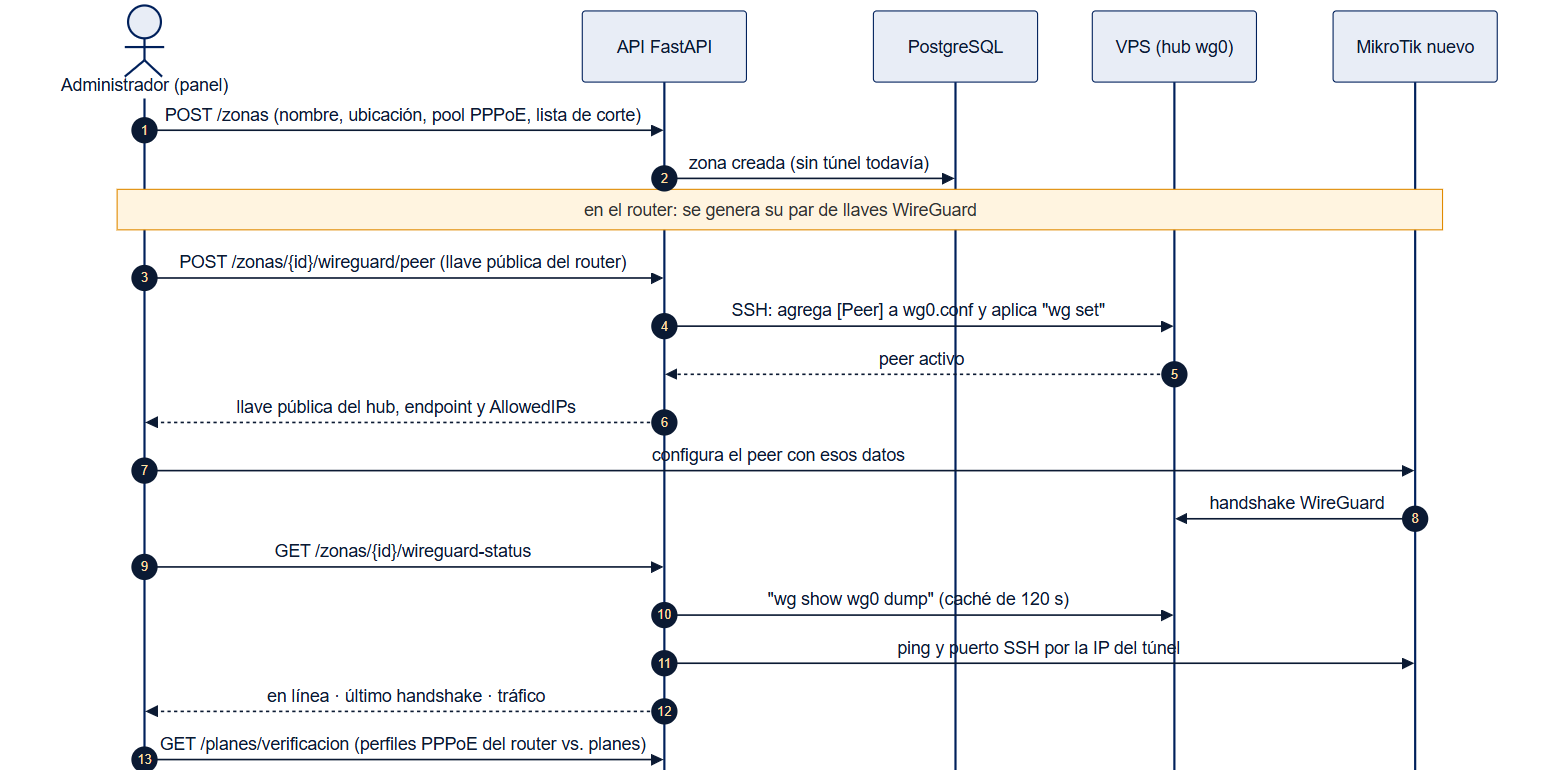
\includegraphics[width=\textwidth,height=0.48\textheight,keepaspectratio]{linea2/d09_alta_zona_wireguard.png}
\caption{Integración con la red: alta de una zona y de su túnel WireGuard desde el panel.}
\label{fig:ce02-e3-zona-wg}
\end{figure}

% ======================================================================
\section{Sección 2: Funcionalidad del sistema}
\label{sec:ce02-e3-func}

\subsection{Mapa del giro del negocio}

La \cref{fig:ce02-e3-mapa} ubica cada parte del sistema en la operación de WISP. El proceso
principal es el ciclo de vida del cliente (pasos 1 a 8); los procesos de gestión fijan las
reglas (planes, zonas, finanzas, accesos) y los de apoyo sostienen pasos concretos del ciclo.

\begin{figure}[H]
\centering
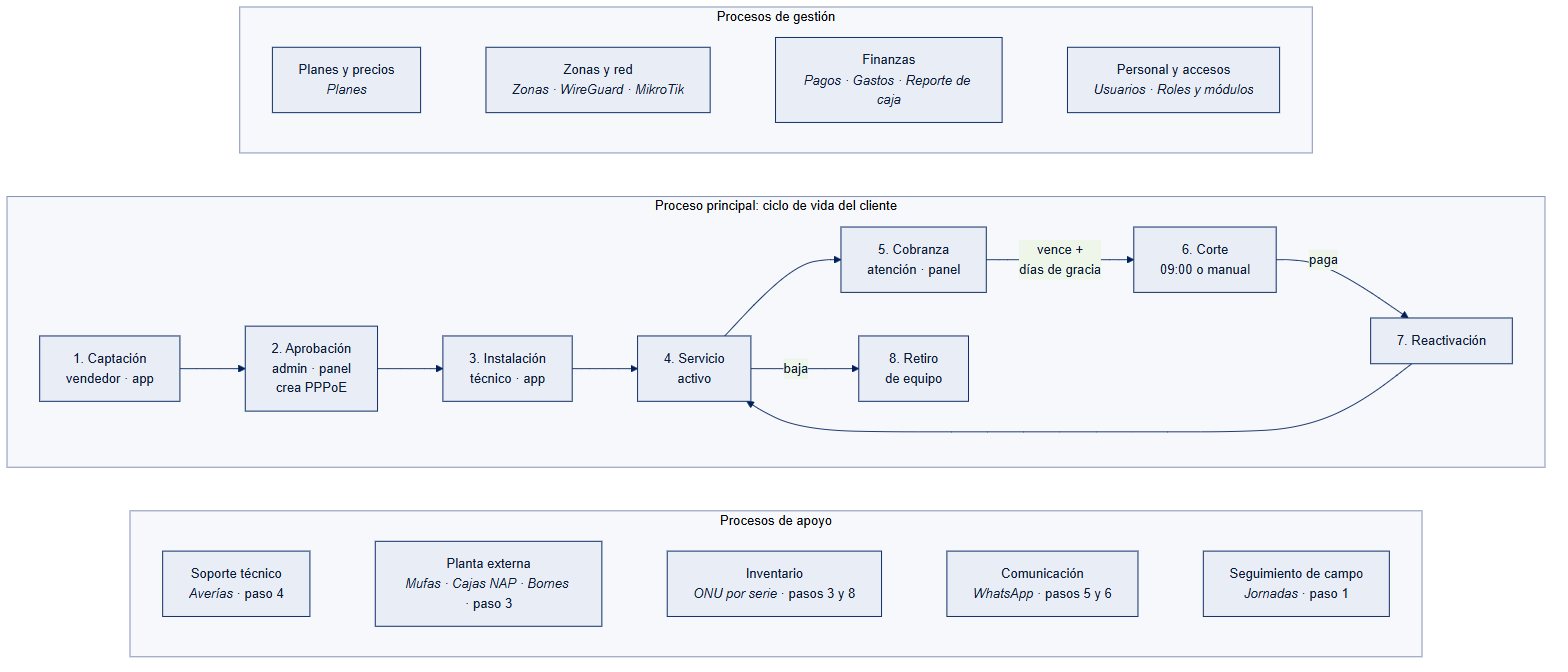
\includegraphics[width=\textwidth]{linea2/d01_mapa_negocio.png}
\caption{Mapa del giro del negocio y módulos del sistema que lo soportan.}
\label{fig:ce02-e3-mapa}
\end{figure}

\subsection{Flujos principales implementados}

\paragraph{Captación, aprobación e instalación.} El vendedor registra al cliente en la app;
el nombre se autocompleta con el DNI y la ubicación se toma del GPS. El administrador aprueba
la venta y en ese momento el sistema crea el secreto PPPoE en el router de la zona. El técnico
de esa zona ve la orden, elige la caja y el borne en el mapa, escanea la ONU y cierra la
instalación con fotos; el cliente queda activo y su fecha de pago se fija desde ese día.

\begin{figure}[H]
\centering
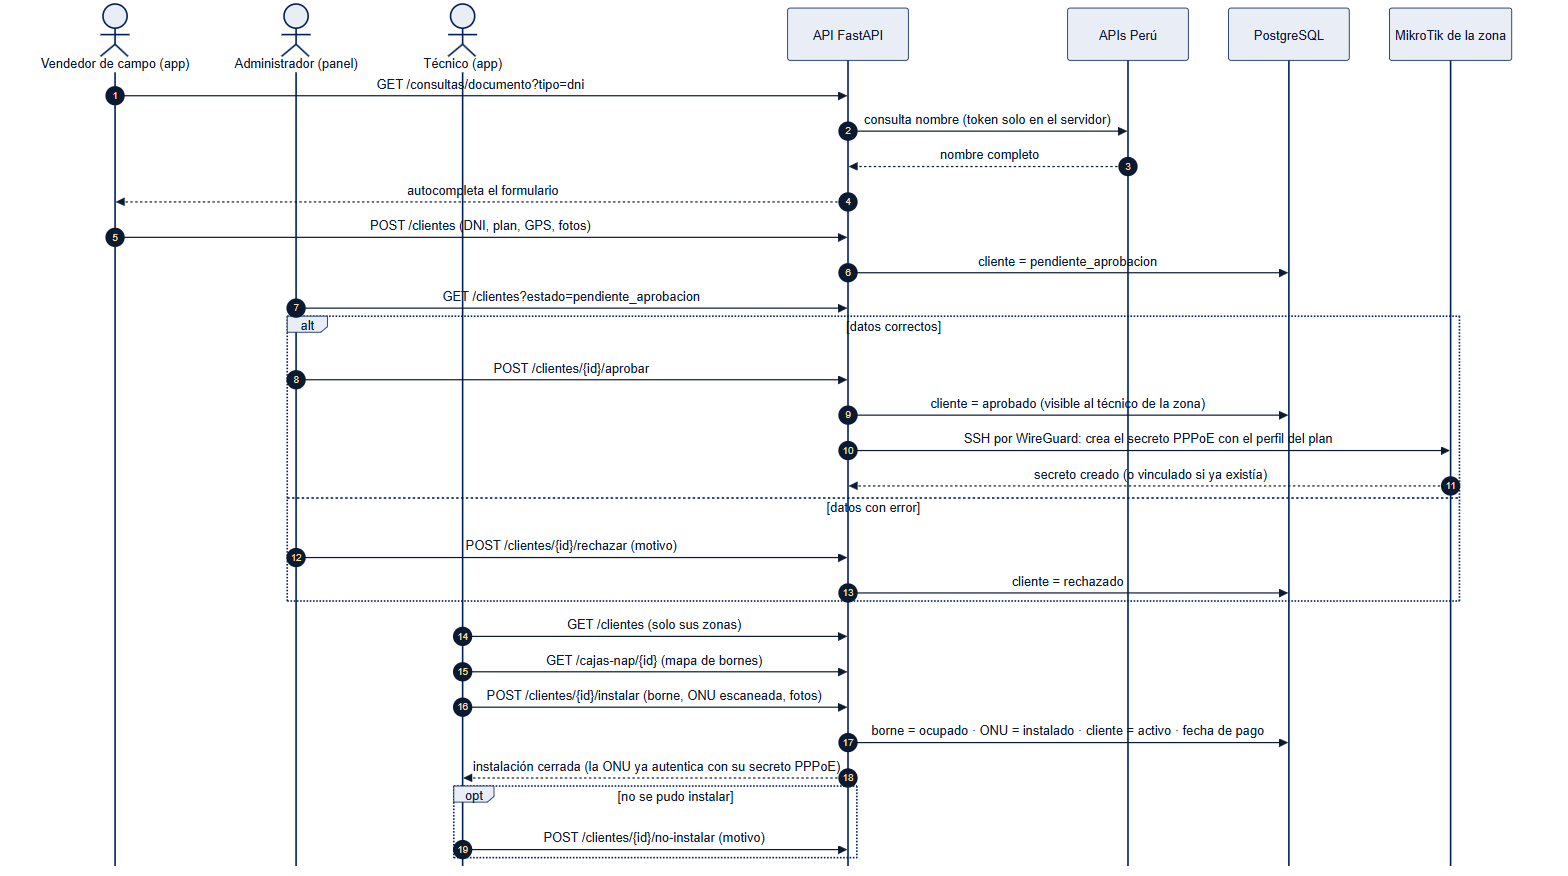
\includegraphics[width=\textwidth,height=0.5\textheight,keepaspectratio]{linea2/d02_venta_instalacion.png}
\caption{Secuencia implementada: captación, aprobación e instalación.}
\label{fig:ce02-e3-venta}
\end{figure}

\paragraph{Cobranza, corte y reactivación.} Cada día a las 08:00 el planificador envía
recordatorios a quienes están por vencer; a las 09:00 corta a los vencidos que superaron los
días de gracia y no tienen un compromiso de pago vigente, avisándoles por WhatsApp
\emph{antes} de cortar. Cuando el cliente paga, atención registra el pago (el número de
operación no puede repetirse), el sistema lo reactiva en el router, extiende su vencimiento
30 días, confirma por WhatsApp y emite el recibo en PDF.

\begin{figure}[H]
\centering
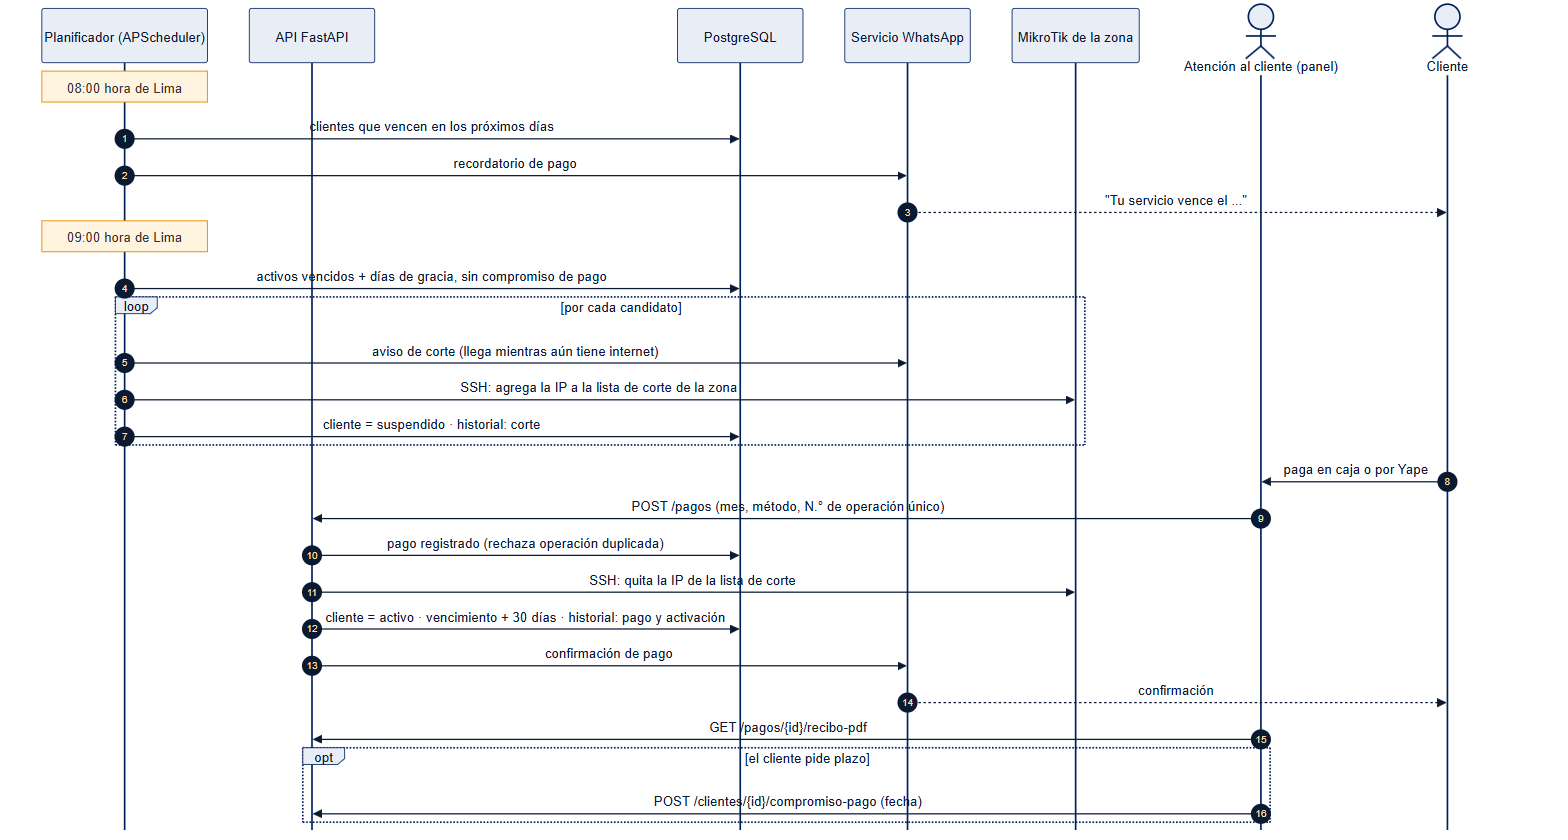
\includegraphics[width=\textwidth,height=0.5\textheight,keepaspectratio]{linea2/d03_cobranza_corte.png}
\caption{Secuencia implementada: recordatorio, corte automático, pago y reactivación.}
\label{fig:ce02-e3-cobranza}
\end{figure}

\paragraph{Averías y retiros.} Las averías pasan por los estados pendiente, asignada, en
proceso y resuelta; si se reemplaza la ONU, el sistema registra la retirada como dañada y la
nueva como instalada. La baja de un cliente genera una orden de retiro: el técnico recoge la
ONU, la roseta y el patchcord, la ONU vuelve al almacén y el borne queda libre.

\begin{figure}[H]
\centering
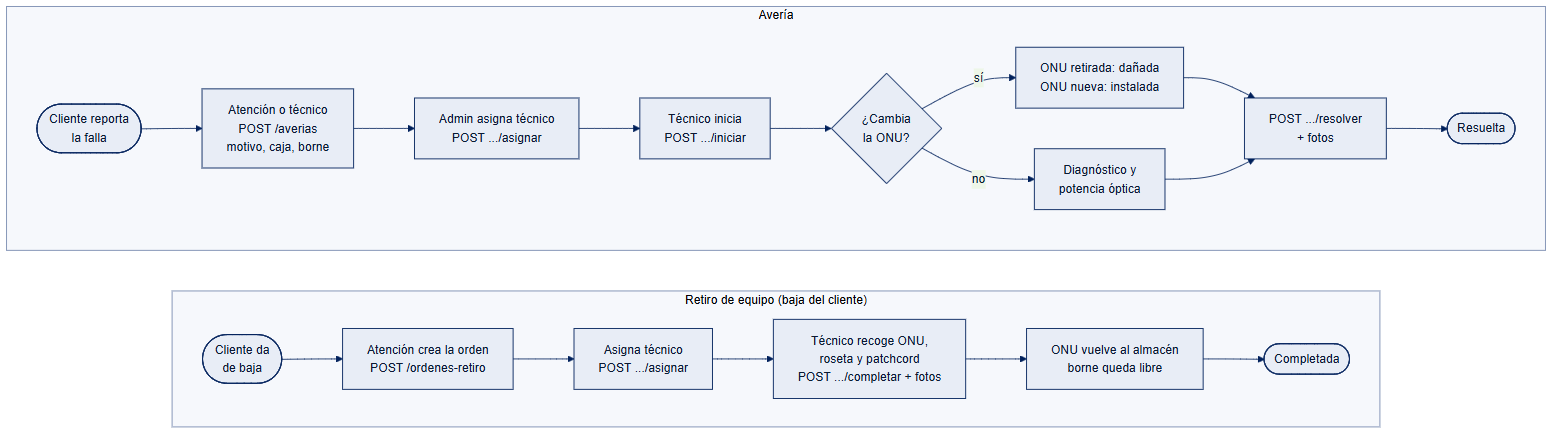
\includegraphics[width=\textwidth]{linea2/d04_averias_retiros.png}
\caption{Flujos implementados de soporte: averías y órdenes de retiro.}
\label{fig:ce02-e3-averias}
\end{figure}

\paragraph{Jornada del vendedor.} Reemplaza la ``ubicación en vivo'' que antes se mandaba al
grupo de WhatsApp: el vendedor inicia su jornada, la app registra puntos del recorrido,
registra sus ventas y al cerrar puede reclamar el pasaje que pagó de su bolsillo; el
administrador ve el recorrido en el mapa y marca el reintegro.

\begin{figure}[H]
\centering
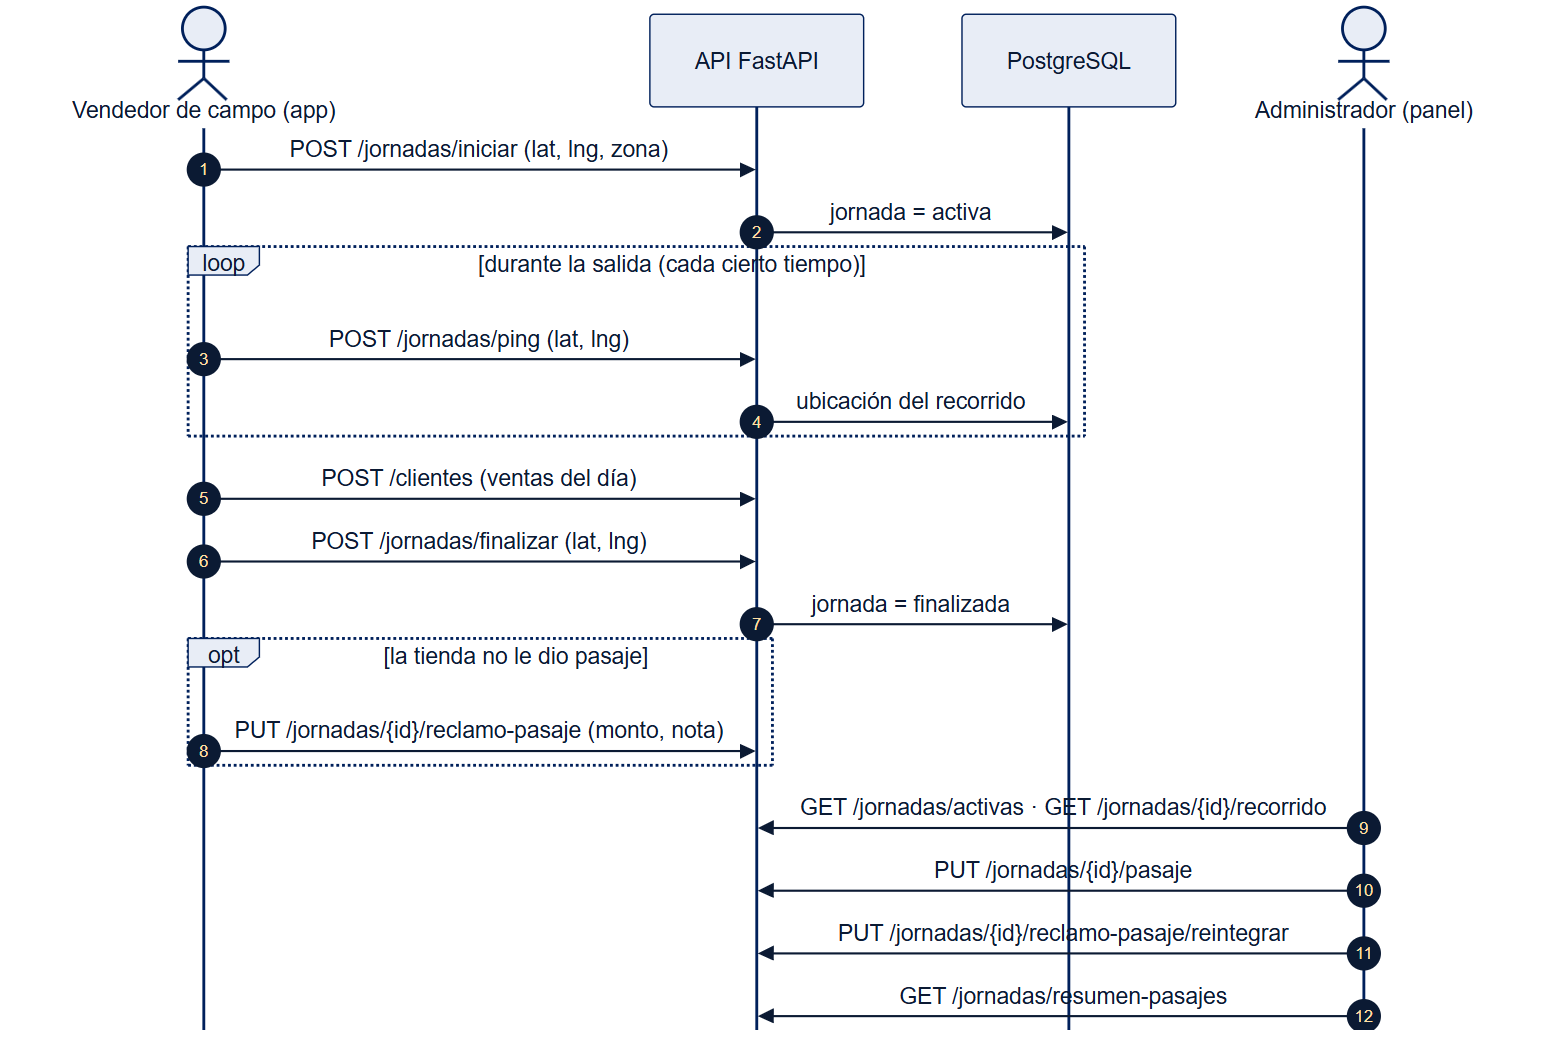
\includegraphics[width=\textwidth,height=0.45\textheight,keepaspectratio]{linea2/d05_jornada_vendedor.png}
\caption{Secuencia implementada: jornada del vendedor y control de pasajes.}
\label{fig:ce02-e3-jornada}
\end{figure}

\subsection{Usuarios, roles y módulos}
\label{sec:ce02-e3-roles}

El acceso combina tres capas que se verifican en cada endpoint: un JWT válido, el
\emph{tipo de cuenta} (\texttt{admin}, \texttt{tecnico}, \texttt{vendedor\_campo},
\texttt{atencion\_cliente}) permitido por \texttt{require\_roles}, y los \emph{módulos} que el
rol tiene asignados, definidos en \texttt{acceso.py}. El administrador puede crear roles,
darles o quitarles módulos uno por uno y ordenar el menú desde el panel, sin tocar el código;
el usuario solo ve en su menú o en su barra inferior los módulos de su rol
(\texttt{GET /api/permisos/mis-modulos}).

\begin{figure}[H]
\centering
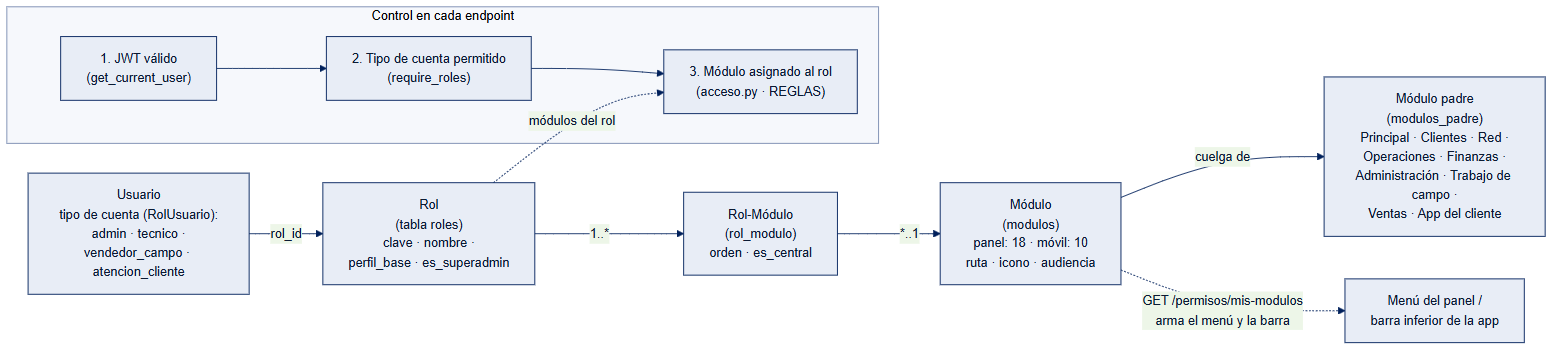
\includegraphics[width=\textwidth]{linea2/d06_roles_modulos.png}
\caption{Modelo de permisos: tipo de cuenta, rol, módulos y control por endpoint.}
\label{fig:ce02-e3-permisos}
\end{figure}

{\small
\begin{longtable}{L{4.2cm}L{2.4cm}L{4.2cm}L{3.6cm}}
\caption{Módulos del panel web (18) y roles que los tienen por defecto.}\label{tab:ce02-e3-mod-panel}\\
\toprule
\textbf{Módulo} & \textbf{Grupo} & \textbf{Ruta} & \textbf{Roles por defecto} \\
\midrule
\endfirsthead
\toprule
\textbf{Módulo} & \textbf{Grupo} & \textbf{Ruta} & \textbf{Roles por defecto} \\
\midrule
\endhead
\bottomrule
\endlastfoot
Dashboard & Principal & \texttt{/dashboard} & Todos los internos \\
Clientes Fibra & Clientes & \texttt{/clientes/fibra} & Admin, atención \\
Clientes Inalámbricos & Clientes & \texttt{/clientes/inalambricos} & Admin, atención \\
Clientes Satelital & Clientes & \texttt{/clientes-satelital} & Admin, atención \\
Pendientes de aprobación & Clientes & \texttt{/clientes/pendientes} & Admin \\
Zonas & Red & \texttt{/zonas} & Admin, atención \\
Cajas NAP & Red & \texttt{/cajas-nap} & Admin \\
Inventario de ONUs & Red & \texttt{/onus} & Admin, atención \\
Averías & Operaciones & \texttt{/averias} & Admin, atención \\
Órdenes de retiro & Operaciones & \texttt{/ordenes-retiro} & Admin, atención \\
Seguimiento de vendedoras & Operaciones & \texttt{/jornadas} & Admin \\
Pagos & Finanzas & \texttt{/pagos} & Admin, atención \\
Gastos & Finanzas & \texttt{/gastos} & Admin \\
Reporte de caja & Finanzas & \texttt{/finanzas/reporte-caja} & Admin \\
Usuarios & Administración & \texttt{/usuarios} & Admin \\
Planes & Administración & \texttt{/planes} & Admin \\
WhatsApp & Administración & \texttt{/configuracion/whatsapp} & Admin \\
Roles y módulos & Administración & \texttt{/configuracion/roles} & Admin \\
\end{longtable}
}

\begin{table}[H]
\centering
\caption{Módulos de la app móvil (10) y barra inferior de cada rol (el módulo central es el botón grande del medio).}
\label{tab:ce02-e3-mod-movil}
\small
\begin{tabularx}{\textwidth}{L{2.6cm}L{2.8cm}X}
\toprule
\textbf{Rol} & \textbf{Grupo} & \textbf{Barra inferior, de izquierda a derecha} \\
\midrule
Técnico & Trabajo de campo & Averías · Retiros · \textbf{Órdenes} (central) · Inventario · Registrar \\
Vendedor de campo & Ventas & Jornada · \textbf{Registrar} (central) · Mis clientes \\
Cliente & App del cliente & Inicio · Pagos · Perfil \\
\bottomrule
\end{tabularx}
\end{table}

\subsection{Panel web}

\begin{figure}[H]
\centering
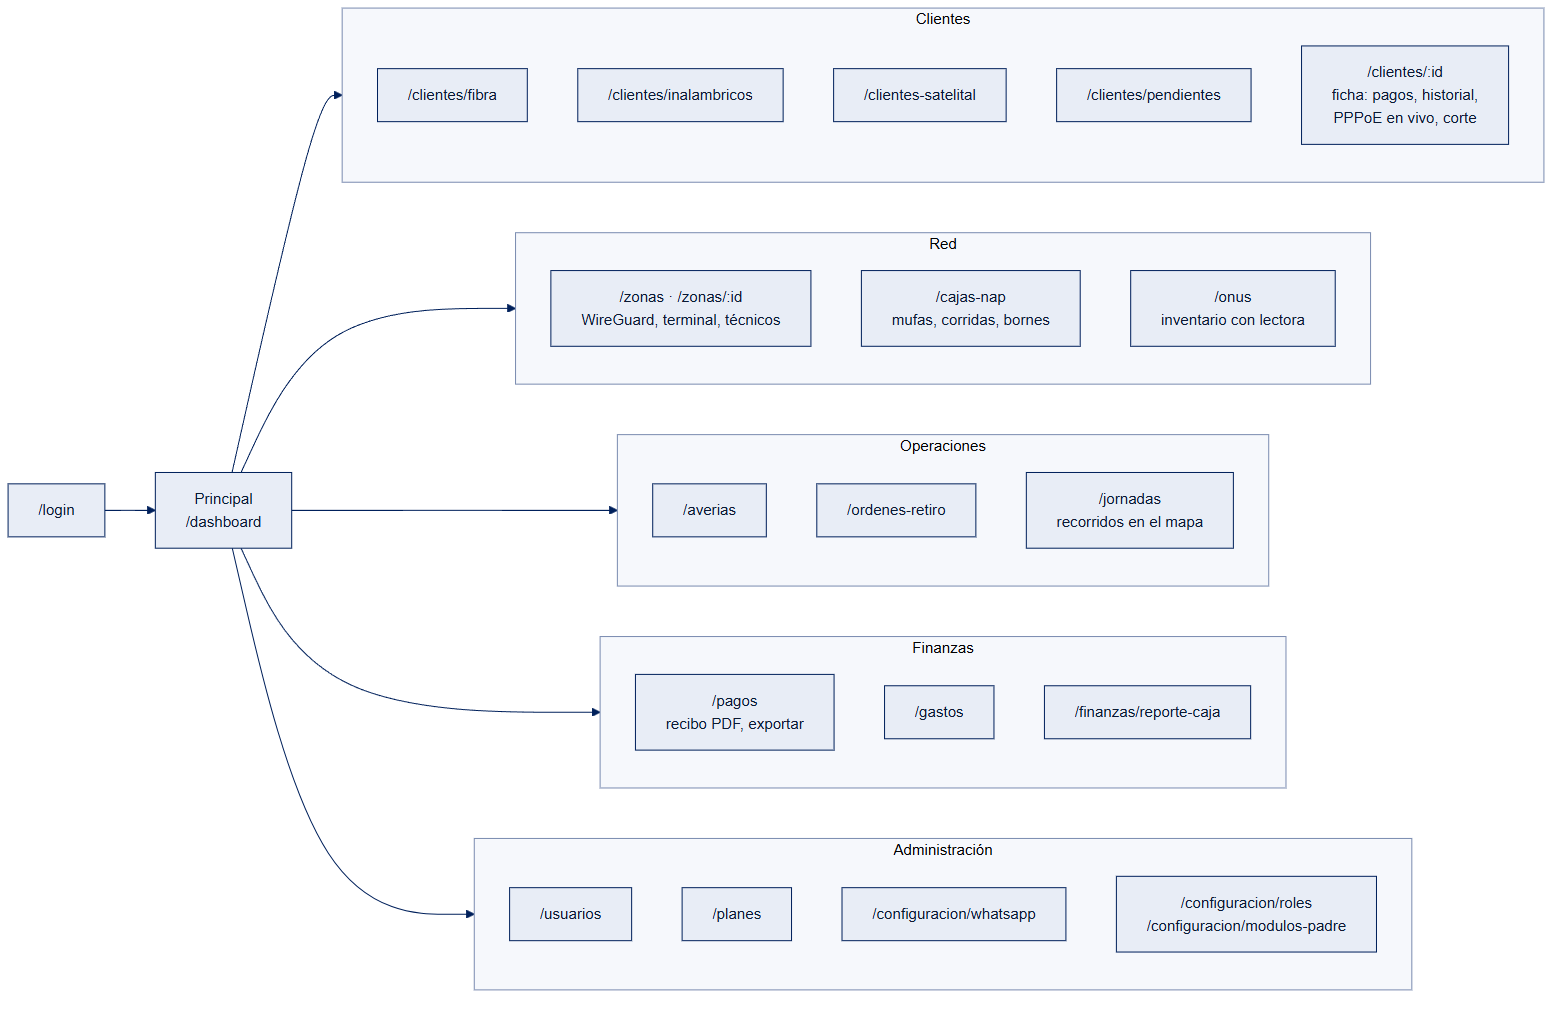
\includegraphics[width=\textwidth,height=0.45\textheight,keepaspectratio]{linea2/d08_panel_web.png}
\caption{Mapa del panel web (\texttt{wispfibra.com/app}) por grupo de menú.}
\label{fig:ce02-e3-panel}
\end{figure}

\begin{table}[H]
\centering
\caption{Funciones principales de cada vista del panel.}
\label{tab:ce02-e3-vistas}
\small
\begin{tabularx}{\textwidth}{L{3.6cm}X}
\toprule
\textbf{Vista} & \textbf{Qué permite hacer} \\
\midrule
Dashboard & Clientes por estado (gráfico de dona), ingresos frente a gastos del año, últimas activaciones y notificaciones calculadas en vivo. \\
Clientes (fibra, inalámbricos, satelital) & Listas con filtros, ficha con calendario anual de pagos, historial, sesión PPPoE en vivo, corte, reactivación, pausa, compromiso de pago y datos de instalación. \\
Pendientes de aprobación & Aprobar (crea el secreto PPPoE) o rechazar con motivo. \\
Zonas & Mapa de cobertura, estado de red de todas las zonas, túnel WireGuard (alta, baja, estado), terminal RouterOS, técnicos asignados y datos del router. \\
Cajas NAP & Mufas, corridas de fibra con metraje y color, cajas y mapa de bornes, ampliación de 8 a 16 bornes, estado PPPoE de los abonados de una caja. \\
Inventario de ONUs & Ingreso con lectora de código de barras, asignación a técnicos, estados e historial. \\
Averías y órdenes de retiro & Registro, asignación, seguimiento por zona y evidencias fotográficas. \\
Seguimiento de vendedoras & Jornadas activas, recorridos en el mapa, pasajes y reintegros. \\
Pagos, gastos y reporte de caja & Registro de pagos y adelantos, recibo PDF, comprobantes, exportación, clientes sin pago, cortados y pausas por vencer, corte de caja del día y recaudación por zona. \\
Usuarios, planes, WhatsApp, roles & Personal, planes sincronizados con los routers (con verificación), vinculación por QR y mensajes masivos, roles y módulos. \\
\bottomrule
\end{tabularx}
\end{table}

\subsection{App móvil}

La app está construida con Expo Router: cada carpeta entre paréntesis es el espacio de un rol
y la pantalla de ingreso deriva al usuario según su tipo de cuenta. Usa la cámara (fotos de
evidencia y escaneo de códigos de barras de las ONU), el GPS (ubicación de la vivienda y
recorrido del vendedor) y la galería, y consume la misma API que el panel
(\texttt{https://wispfibra.com/api}).

\begin{figure}[H]
\centering
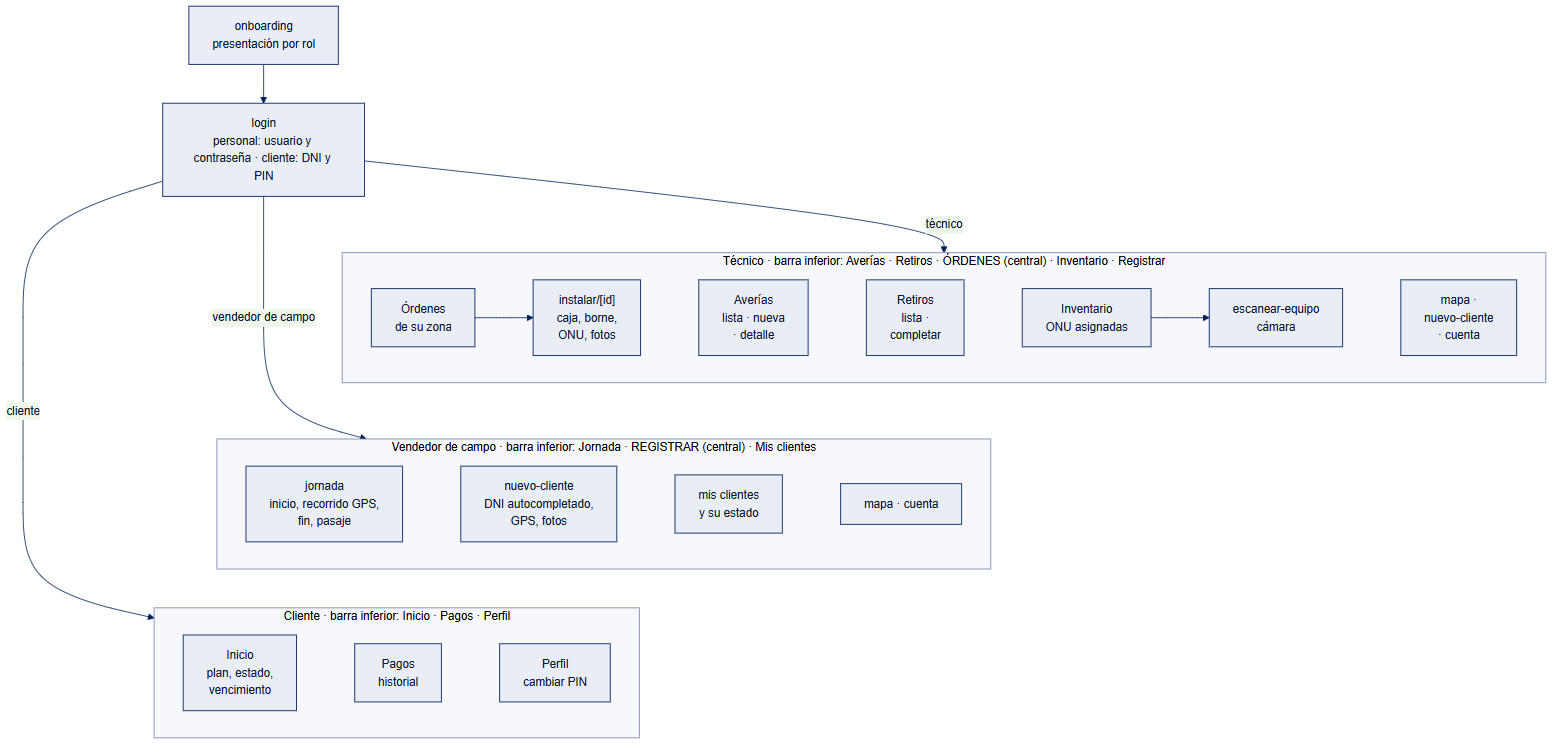
\includegraphics[width=\textwidth,height=0.5\textheight,keepaspectratio]{linea2/d07_app_movil.png}
\caption{Navegación de la app móvil por rol.}
\label{fig:ce02-e3-movil}
\end{figure}

{\small
\begin{longtable}{L{4.6cm}L{1.8cm}L{7.6cm}}
\caption{Pantallas de la app móvil (28 archivos de Expo Router).}\label{tab:ce02-e3-pantallas}\\
\toprule
\textbf{Pantalla} & \textbf{Rol} & \textbf{Función} \\
\midrule
\endfirsthead
\toprule
\textbf{Pantalla} & \textbf{Rol} & \textbf{Función} \\
\midrule
\endhead
\bottomrule
\endlastfoot
\texttt{onboarding} & Todos & Presentación inicial según el tipo de usuario. \\
\texttt{(auth)/login} & Todos & Ingreso del personal (usuario y contraseña) o del cliente (DNI y PIN). \\
\texttt{(tecnico)/index}, \texttt{instalaciones} & Técnico & Órdenes aprobadas de sus zonas. \\
\texttt{(tecnico)/instalar/[id]} & Técnico & Caja NAP, borne, ONU, precinto, potencia y fotos; cierre o ``no se pudo instalar''. \\
\texttt{(tecnico)/averias/index, nueva, [id]} & Técnico & Lista, registro y atención de averías hasta resolverlas. \\
\texttt{(tecnico)/retiros/index, [id]} & Técnico & Órdenes de retiro y confirmación del equipo recogido. \\
\texttt{(tecnico)/inventario} & Técnico & ONU asignadas, marcar dañada o devolver. \\
\texttt{(tecnico)/escanear-equipo} & Técnico & Escaneo del código de barras de la ONU con la cámara. \\
\texttt{(tecnico)/mapa} & Técnico & Mapa de cajas NAP y clientes. \\
\texttt{(tecnico)/nuevo-cliente}, \texttt{cuenta} & Técnico & Registrar un cliente y datos de la cuenta. \\
\texttt{(vendedor)/index}, \texttt{cliente/[id]} & Vendedor & Mis clientes y el estado de cada venta. \\
\texttt{(vendedor)/nuevo-cliente} & Vendedor & Registro con DNI autocompletado, GPS y fotos. \\
\texttt{(vendedor)/jornada} & Vendedor & Iniciar y cerrar la jornada, recorrido y reclamo de pasaje. \\
\texttt{(vendedor)/mapa}, \texttt{cuenta} & Vendedor & Mapa de cobertura y datos de la cuenta. \\
\texttt{(cliente)/index} & Cliente & Plan, estado del servicio y vencimiento. \\
\texttt{(cliente)/pagos} & Cliente & Historial de pagos. \\
\texttt{(cliente)/perfil} & Cliente & Datos y cambio de PIN. \\
\end{longtable}
}

\subsection{Sitio público}

El sitio \texttt{wispfibra.com} muestra los planes, los beneficios, la cobertura y las preguntas
frecuentes, y tiene accesos a ``Ingresar'' (panel) y ``Contratar''. Las cifras de cobertura no
están escritas a mano: salen de los endpoints públicos \texttt{/api/zonas/publicas} y
\texttt{/api/zonas/publicas/resumen}.

\begin{figure}[H]
\centering
\begin{minipage}[t]{0.68\textwidth}\centering

\includegraphics[width=\linewidth]{linea2/cap_sitio_publico.png}
\end{minipage}\hfill
\begin{minipage}[t]{0.27\textwidth}\centering

\includegraphics[width=\linewidth]{linea2/cap_sitio_movil.png}
\end{minipage}
\caption{Sitio público en producción, 19/11/2026: versión de escritorio y de celular.}
\label{fig:ce02-e3-sitio}
\end{figure}

\subsection{Automatizaciones y notificaciones}

\begin{table}[H]
\centering
\caption{Procesos automáticos del sistema.}
\label{tab:ce02-e3-automaticos}
\small
\begin{tabularx}{\textwidth}{L{3.4cm}L{2.6cm}X}
\toprule
\textbf{Proceso} & \textbf{Cuándo} & \textbf{Qué hace} \\
\midrule
Recordatorio preventivo & 08:00 diario (Lima) & Avisa por WhatsApp a quienes vencen en los próximos días; también se puede lanzar a mano. \\
Corte automático & 09:00 diario (Lima) & Corta a los vencidos que superaron los días de gracia, salvo compromiso de pago vigente; avisa antes del corte. \\
Reactivación & Al registrar un pago & Quita al cliente de la lista de corte del router y extiende su vencimiento. \\
Confirmación de pago & Al registrar un pago & Mensaje de WhatsApp con el detalle; se puede reenviar. \\
Mensajes masivos & A pedido & Envío por zona y estado con pausas aleatorias y registro por destinatario. \\
Notificaciones del panel & En cada consulta & Ventas por aprobar, instalaciones recientes o fallidas, averías demoradas y estado de WhatsApp, calculadas en vivo. \\
\bottomrule
\end{tabularx}
\end{table}

\subsection{Evidencias funcionales}

\begin{table}[H]
\centering
\caption{Verificación del sistema en producción (19/11/2026, consulta de cabeceras HTTP).}
\label{tab:ce02-e3-verificacion}
\small
\begin{tabularx}{\textwidth}{L{5cm}L{1.6cm}X}
\toprule
\textbf{URL} & \textbf{Respuesta} & \textbf{Observación} \\
\midrule
\texttt{https://wispfibra.com/} & 200 OK & Sitio público; servidor Cloudflare; HSTS de un año. \\
\texttt{https://www.wispfibra.com/} & 200 OK & Mismo sitio por el subdominio \texttt{www}. \\
\texttt{https://wispfibra.com/app/} & 200 OK & Pantalla de ingreso del panel (\cref{fig:ce02-e3-login}). \\
\texttt{https://wispfibra.com/api/health} & 200 OK & La API responde a través del túnel. \\
\bottomrule
\end{tabularx}
\end{table}

\begin{figure}[H]
\centering

\includegraphics[width=0.62\textwidth]{linea2/cap_panel_login.png}
\caption{Pantalla de ingreso del panel en producción (\texttt{wispfibra.com/app}).}
\label{fig:ce02-e3-login}
\end{figure}

\subsubsection*{Pantallas internas del panel}

Las siguientes capturas se tomaron el 19/11/2026 del mismo sistema ejecutado en un entorno
local con Docker (\texttt{docker-compose.local.yml}), con datos de prueba. Antes de cada
captura se anonimizaron en pantalla los nombres, DNI, teléfonos, direcciones, usuarios PPPoE,
correos y coordenadas; los valores que se ven (``Cliente Demo 02'', ``\textbullet\textbullet\textbullet'') son ficticios.

\begin{figure}[H]
\centering
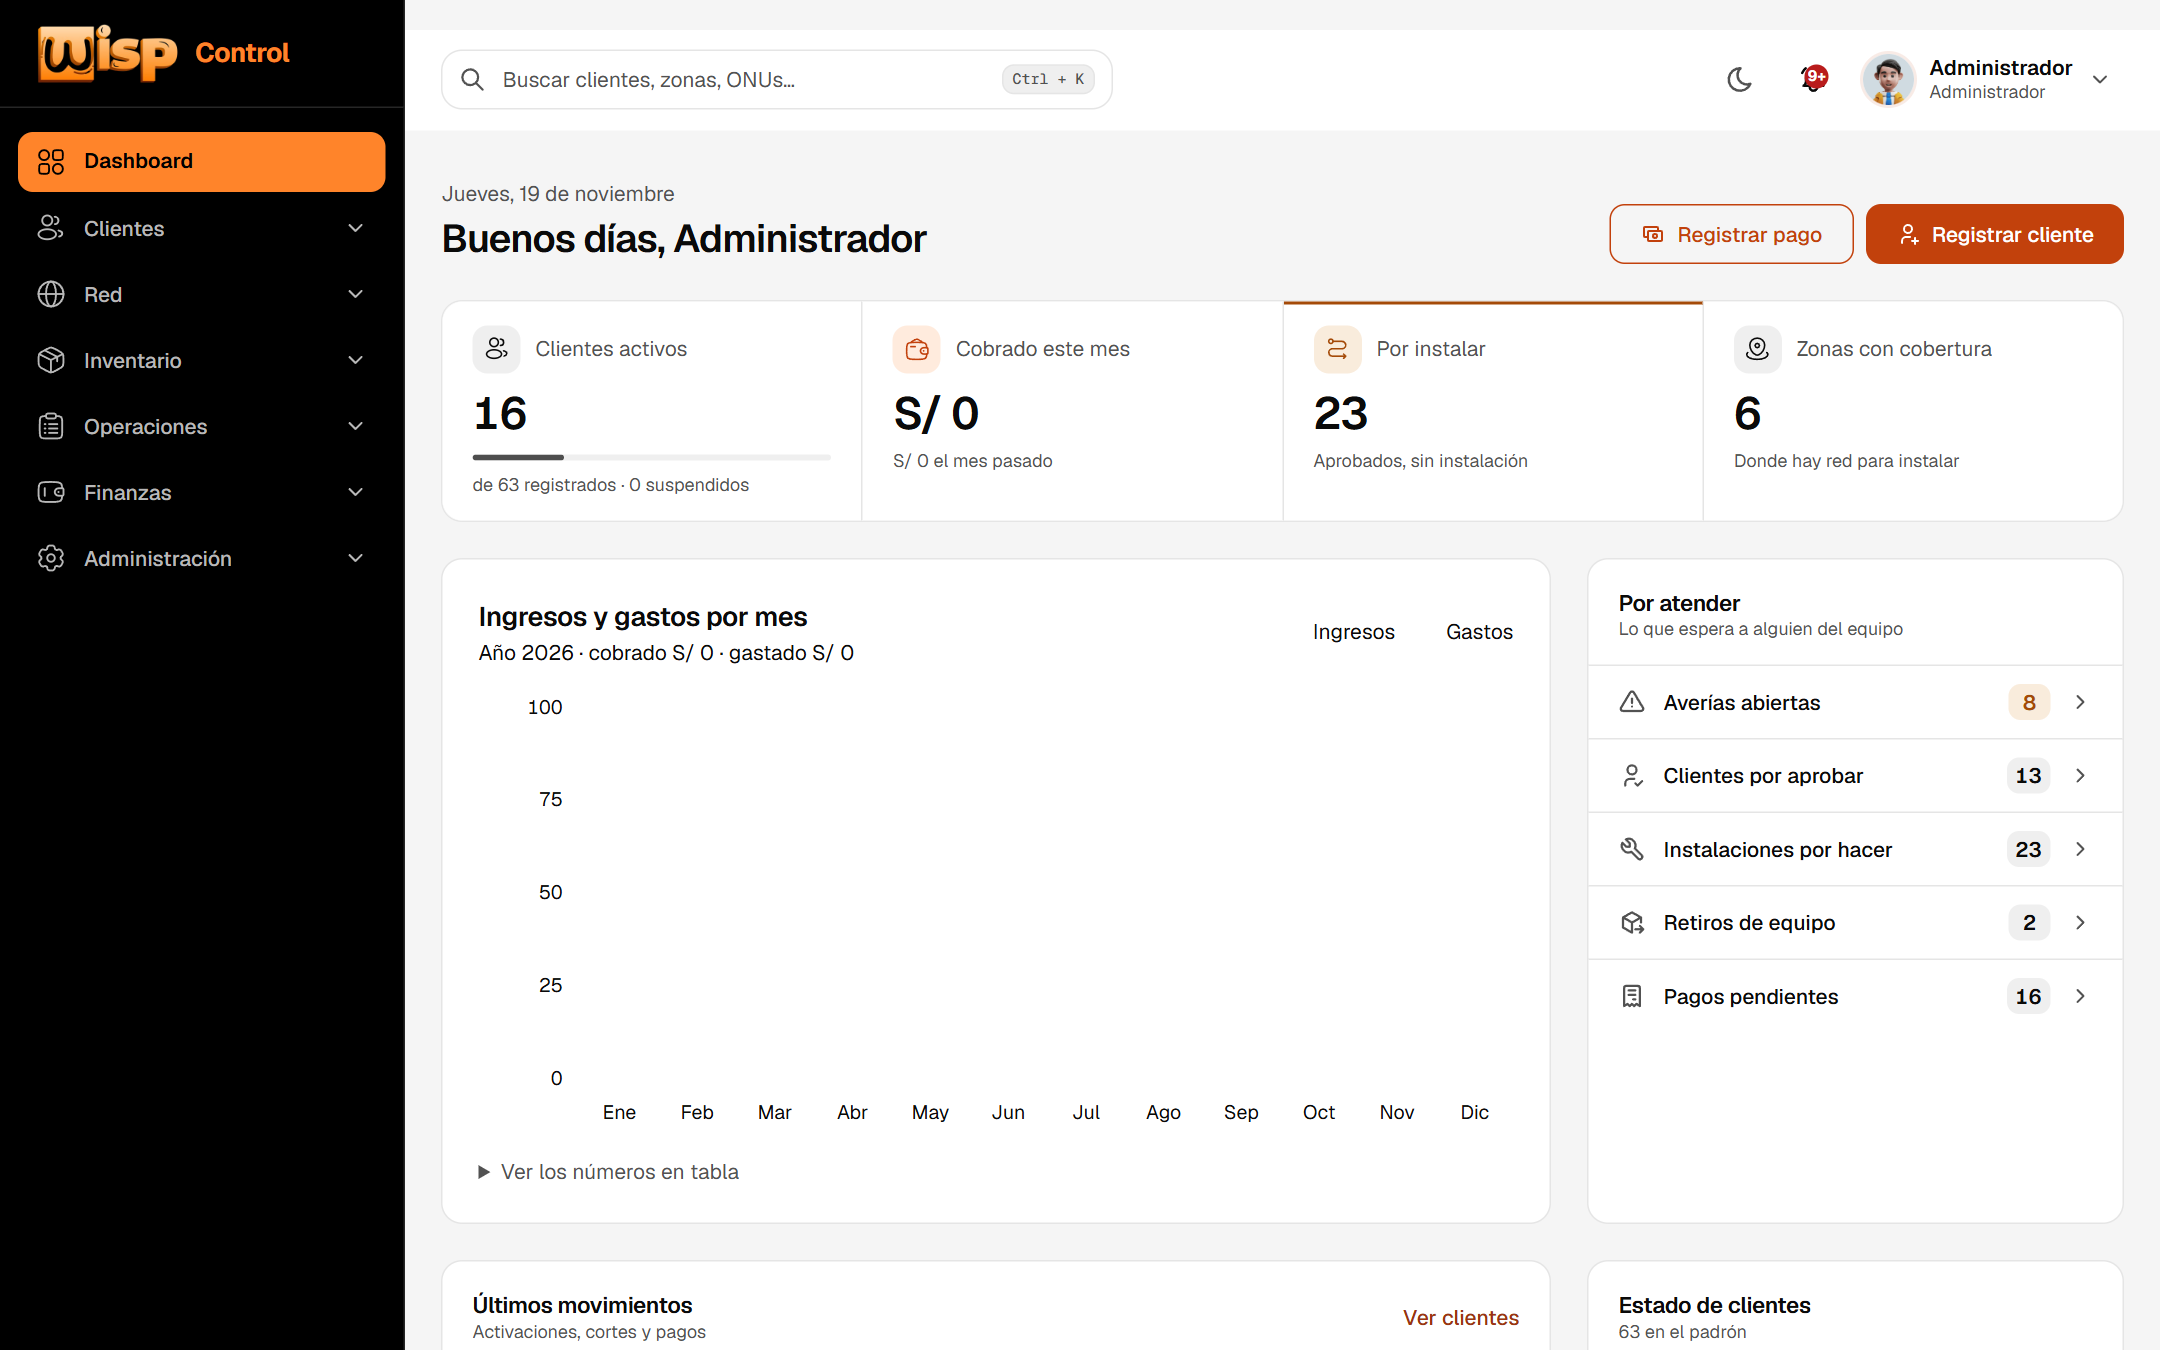
\includegraphics[width=\textwidth]{linea2/panel/p01_dashboard.png}
\caption{Dashboard: indicadores del mes y bandeja \emph{Por atender} con averías, aprobaciones, instalaciones, retiros y pagos pendientes.}
\label{fig:ce02-e3-dashboard}
\end{figure}

\begin{figure}[H]
\centering
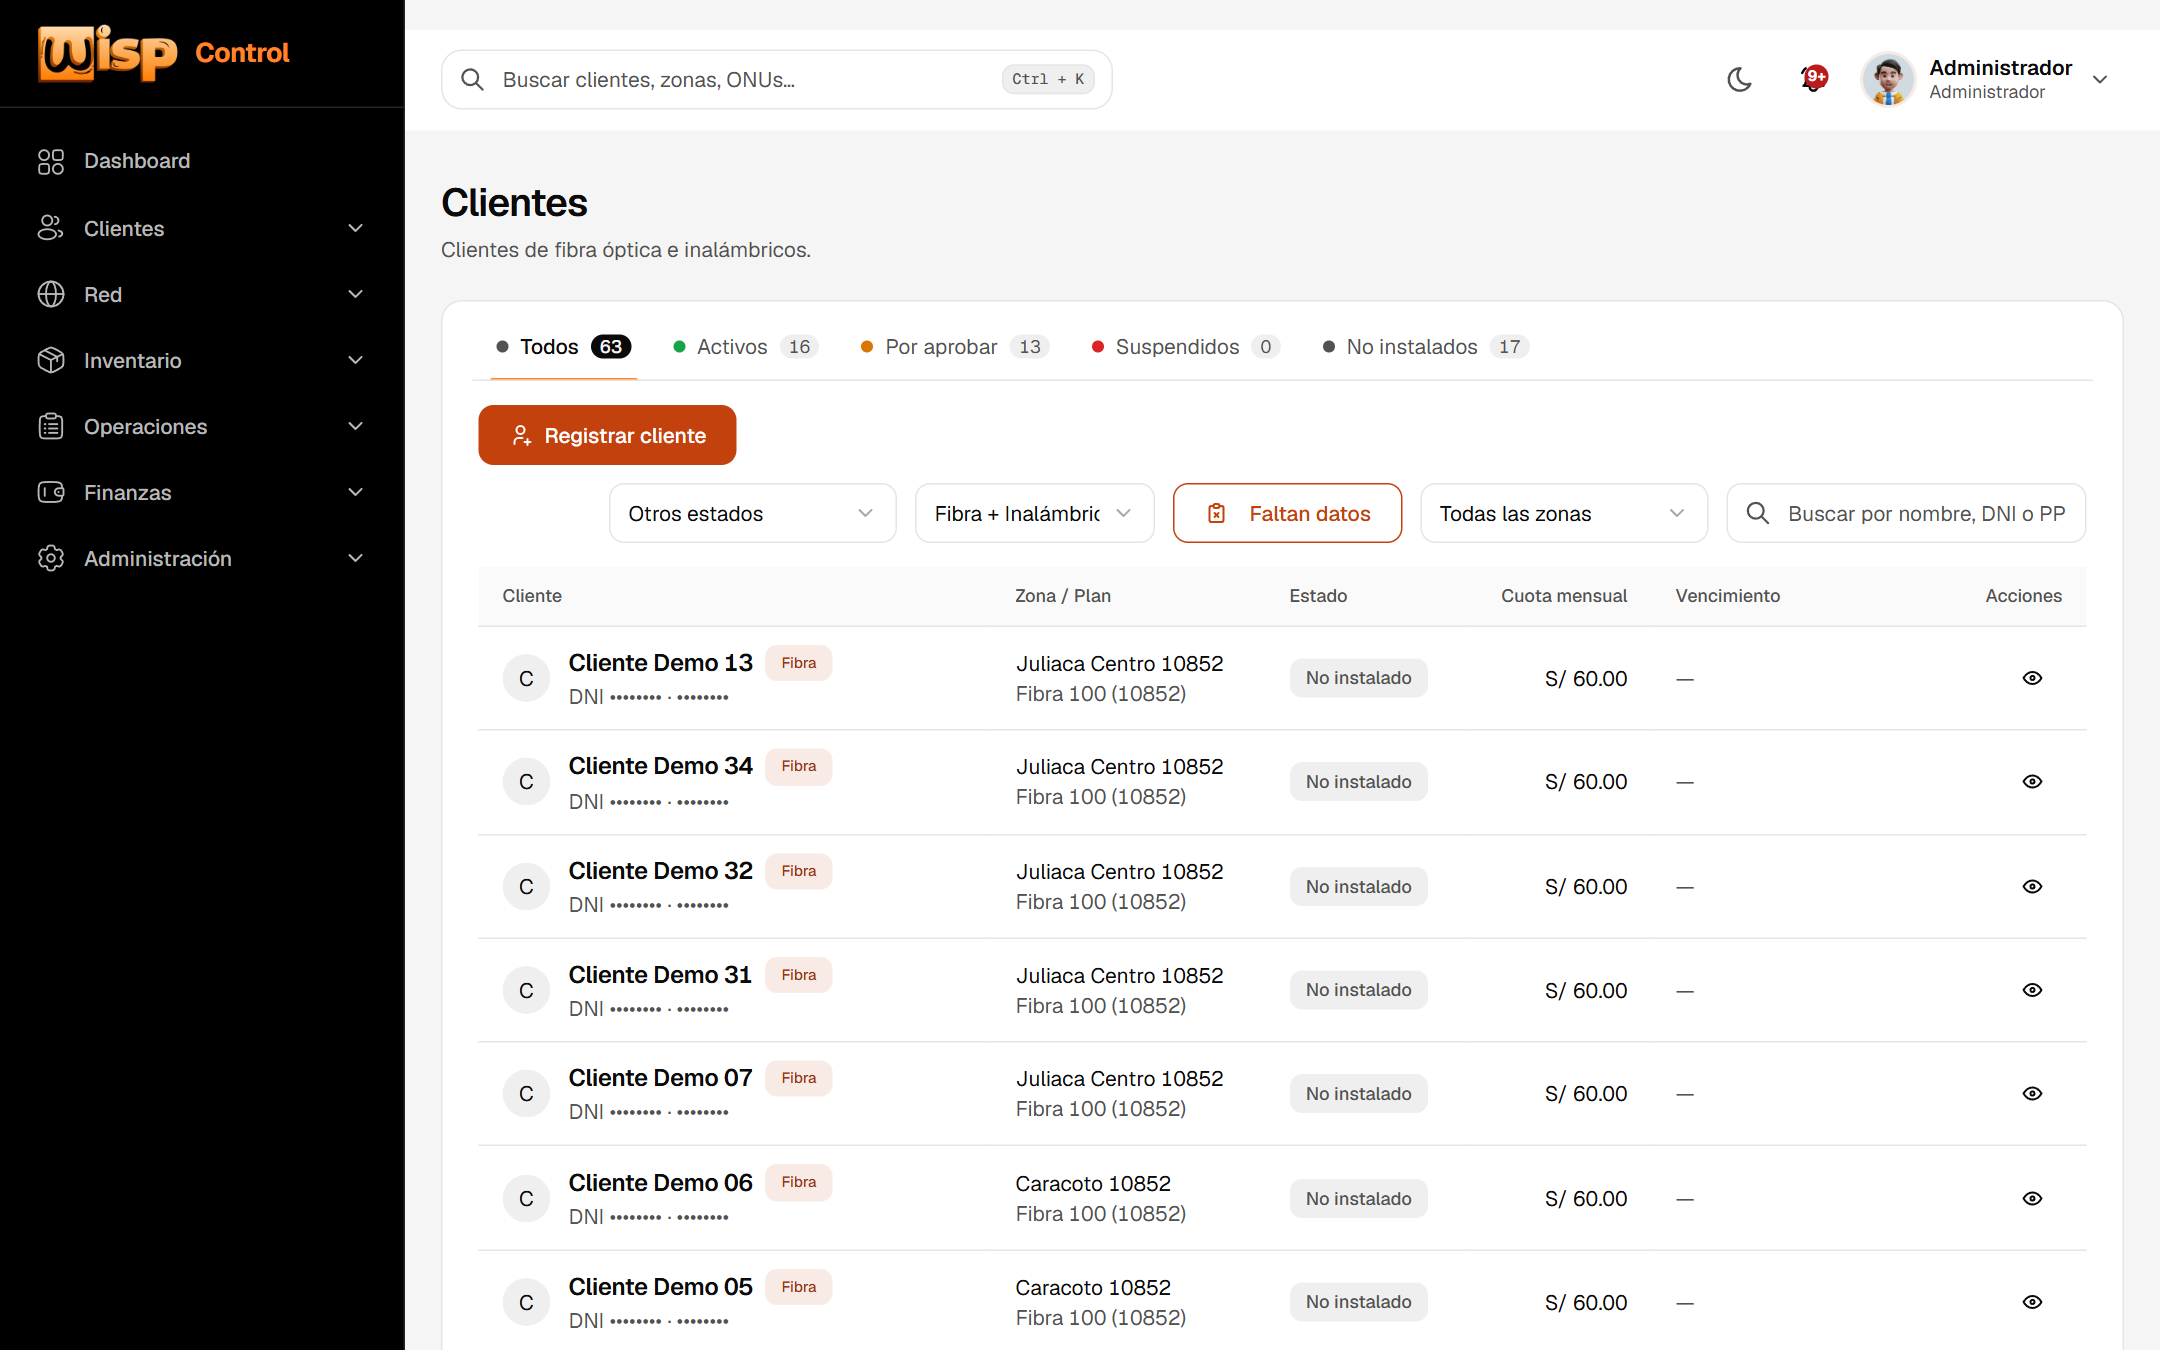
\includegraphics[width=\textwidth]{linea2/panel/p02_clientes.png}
\caption{Padrón de clientes con pestañas por estado, filtros por tipo y zona, y búsqueda por nombre, DNI o usuario PPPoE.}
\label{fig:ce02-e3-clientes}
\end{figure}

\begin{figure}[H]
\centering
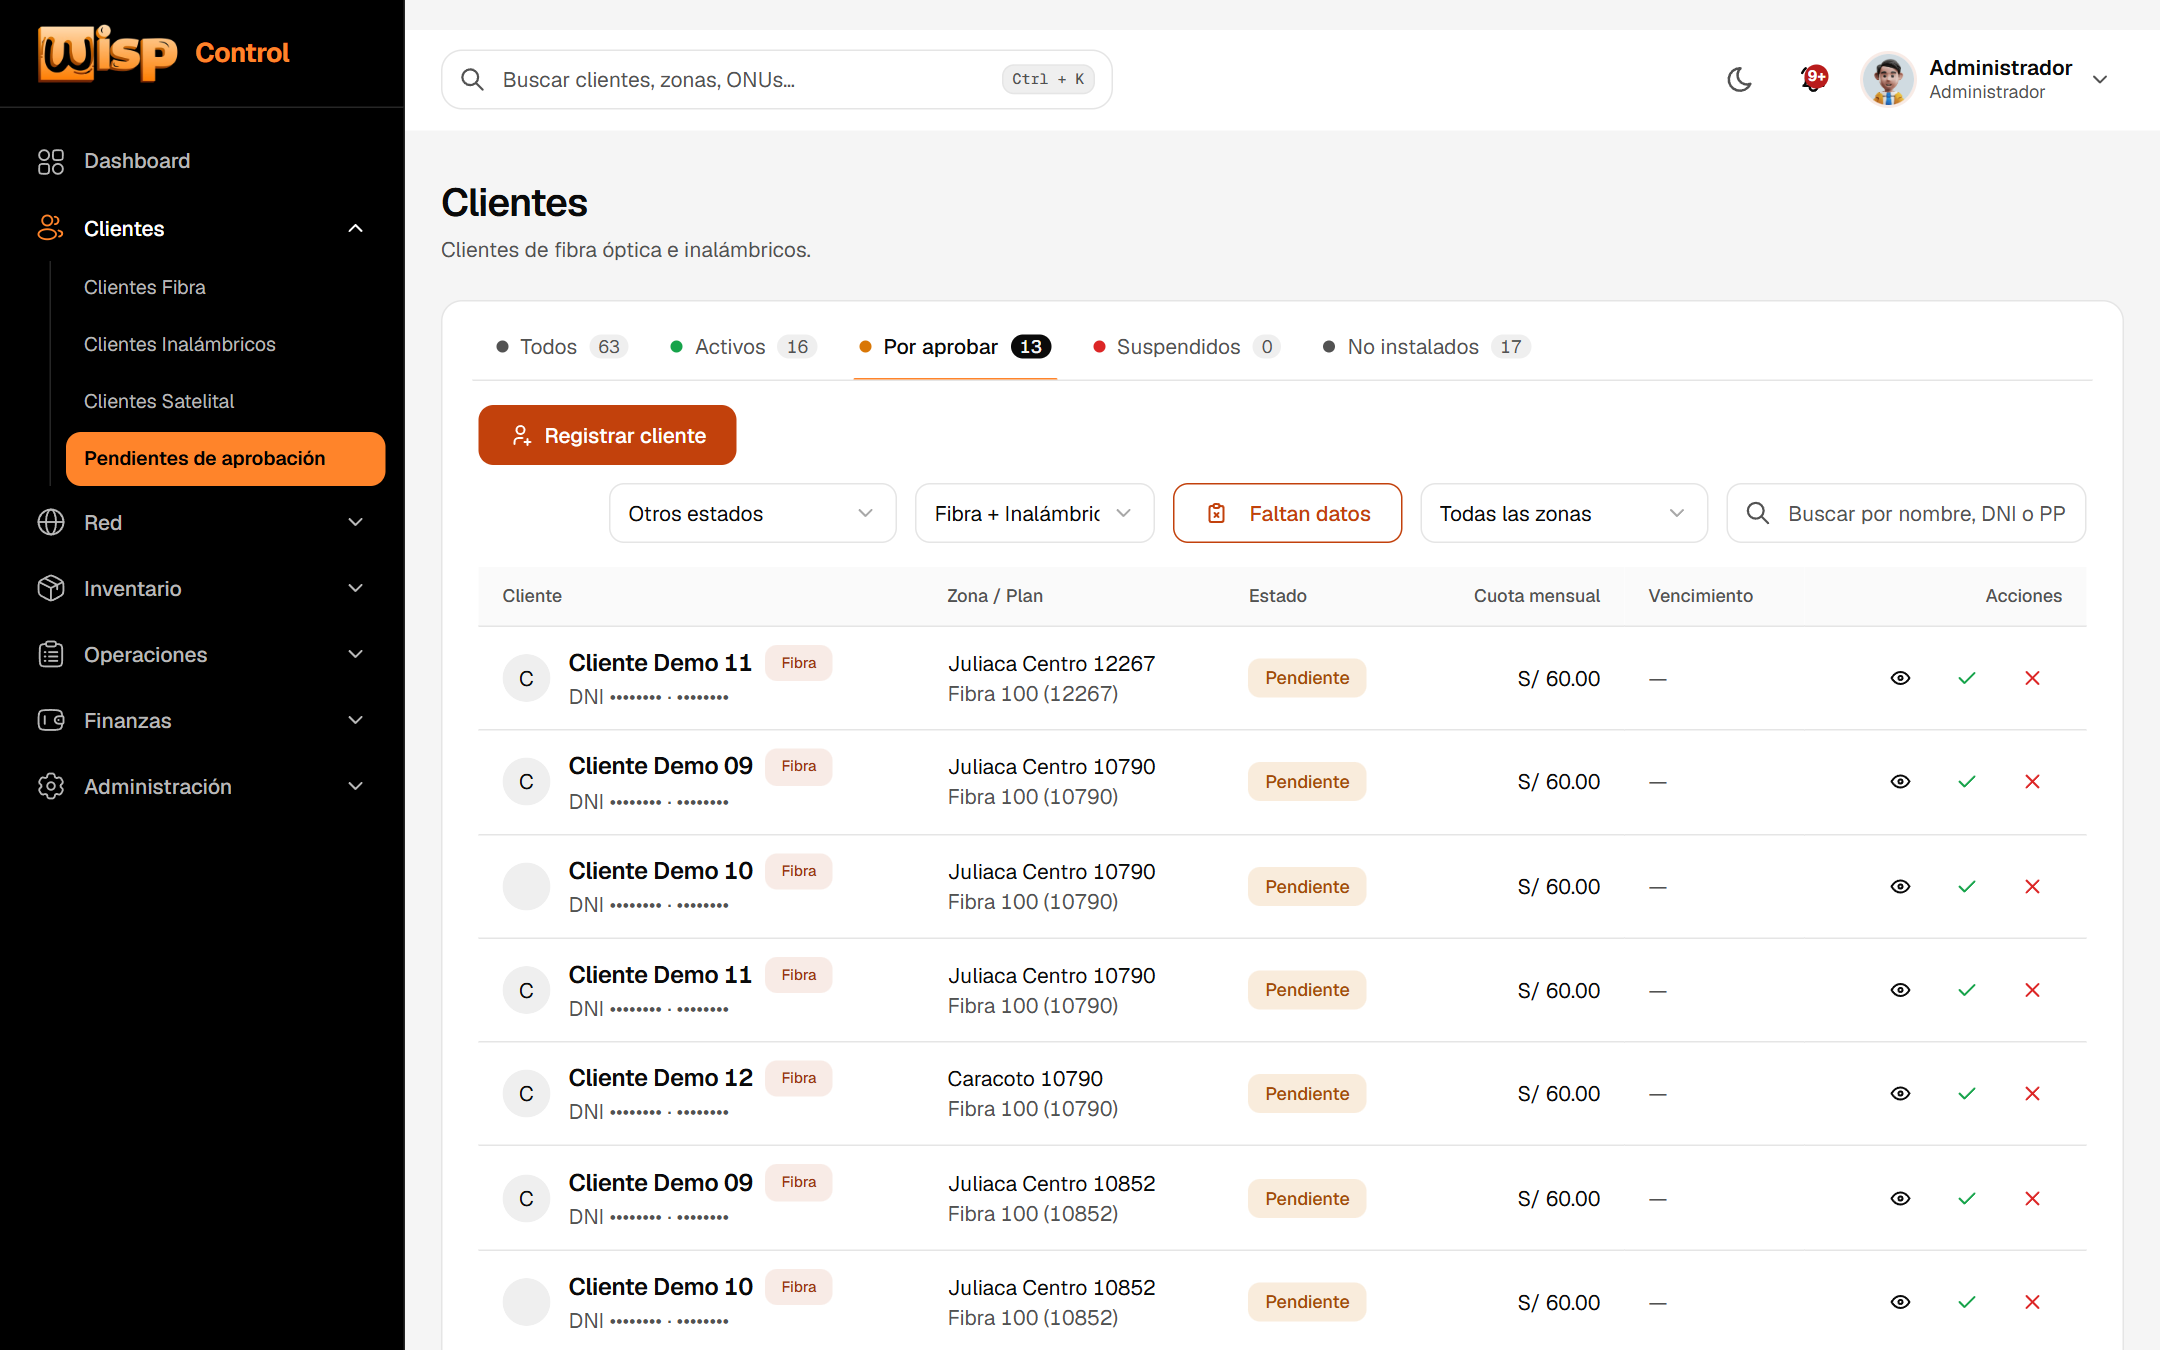
\includegraphics[width=\textwidth]{linea2/panel/p14_pendientes.png}
\caption{Clientes pendientes de aprobación: la venta registrada en campo se aprueba o rechaza desde aquí; al aprobar se crea el secreto PPPoE.}
\label{fig:ce02-e3-pendientes}
\end{figure}

\begin{figure}[H]
\centering
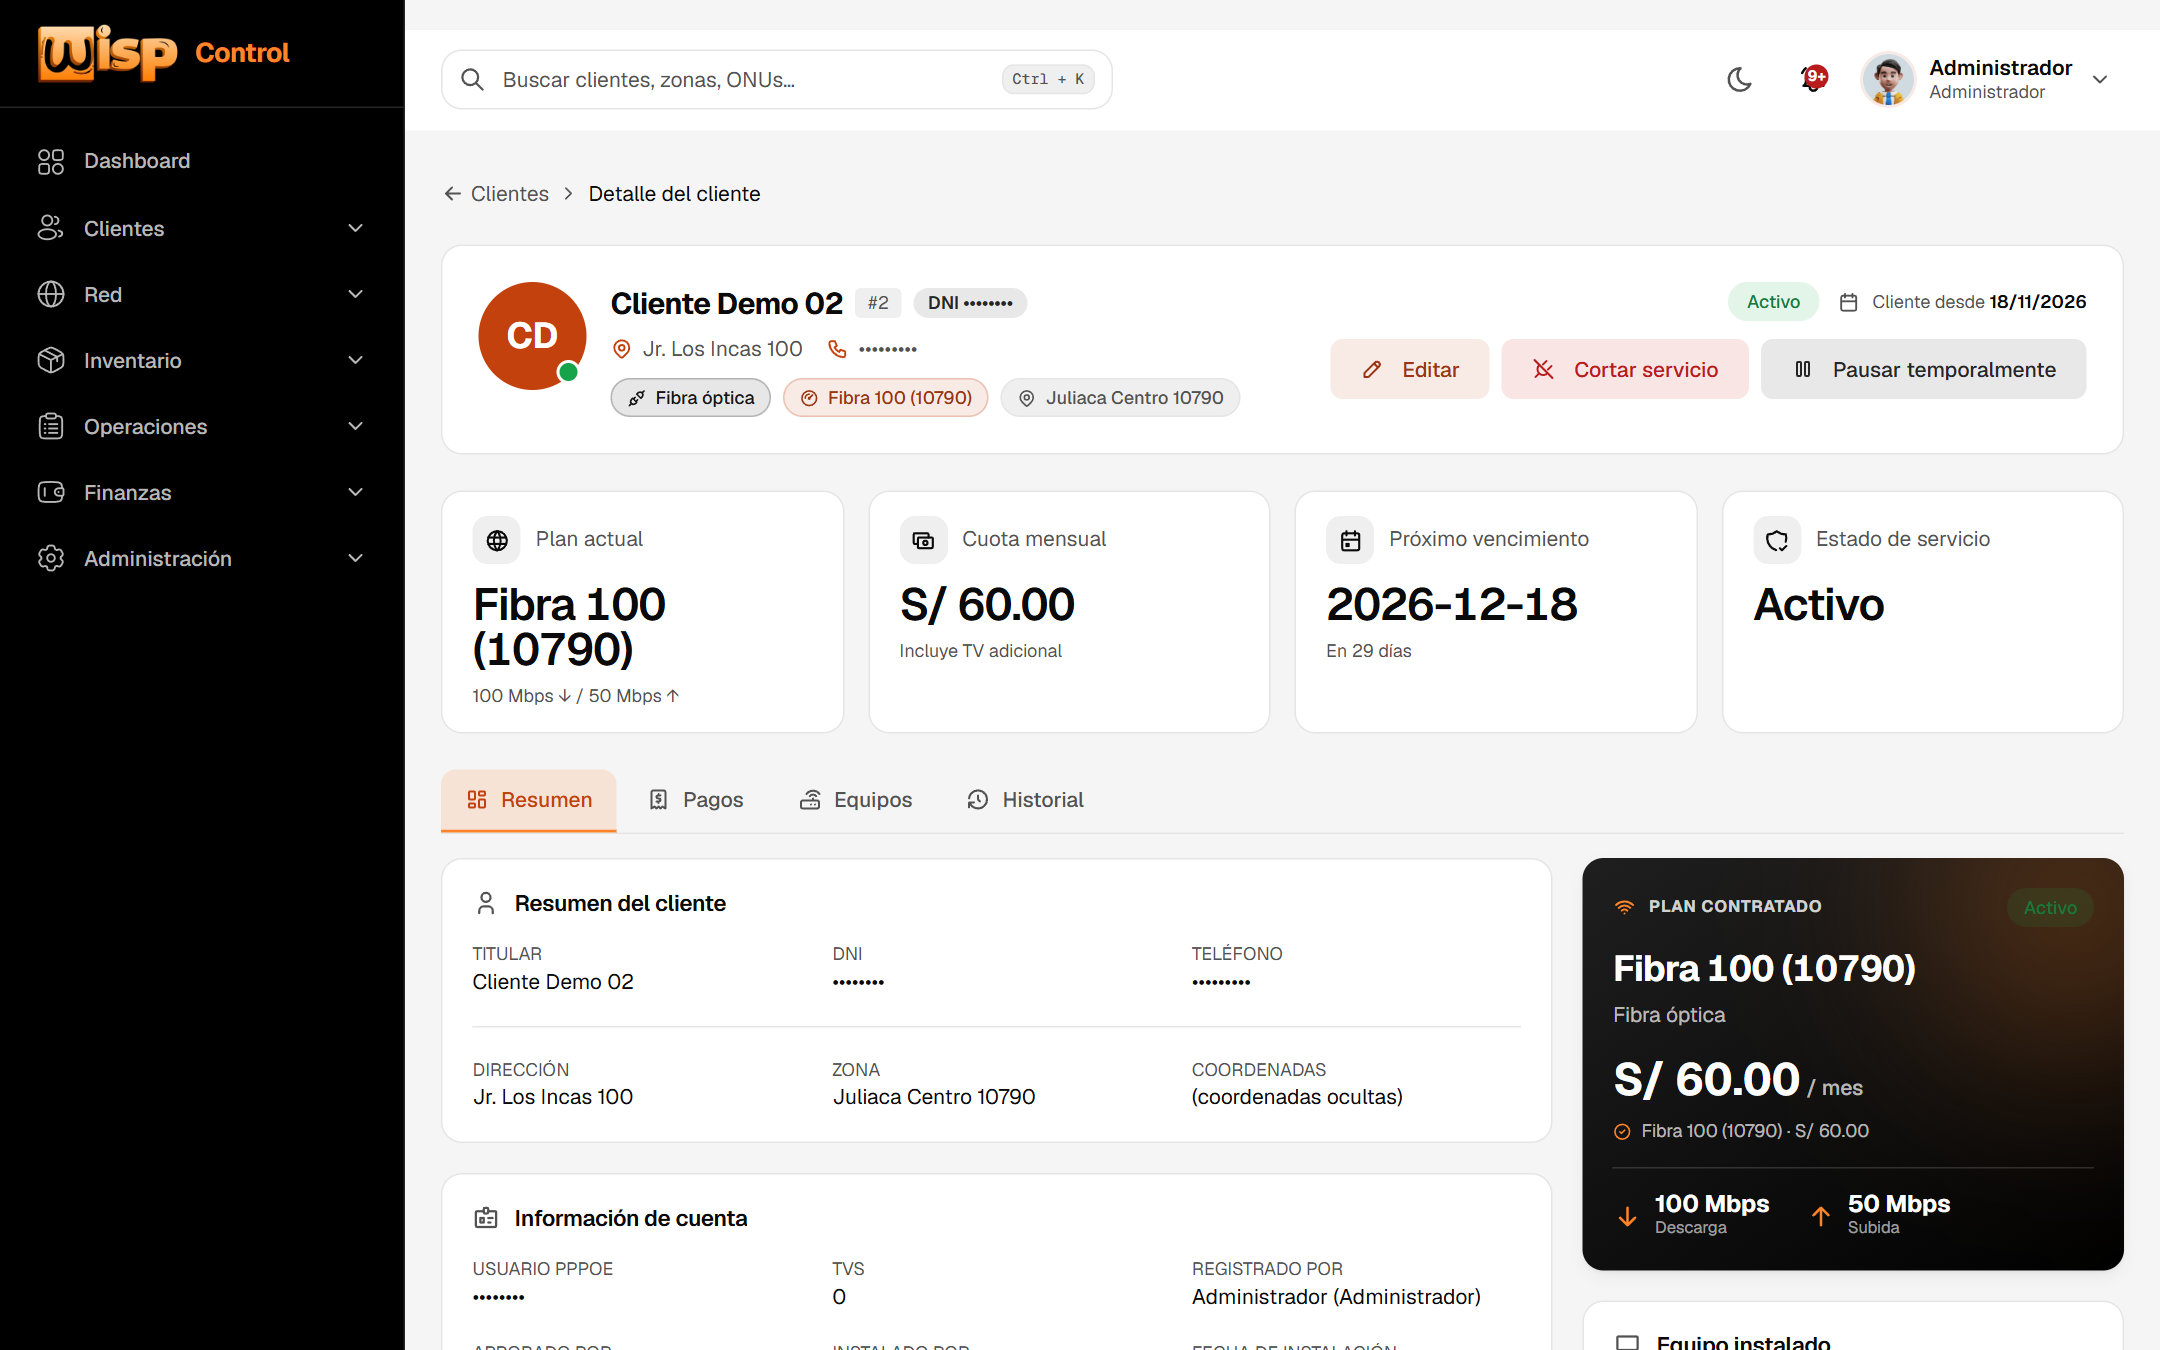
\includegraphics[width=\textwidth]{linea2/panel/p03_cliente_detalle.png}
\caption{Ficha del cliente: plan, cuota, vencimiento, estado y acciones de corte y pausa; pestañas de pagos, equipos e historial.}
\label{fig:ce02-e3-cliente-detalle}
\end{figure}

\begin{figure}[H]
\centering
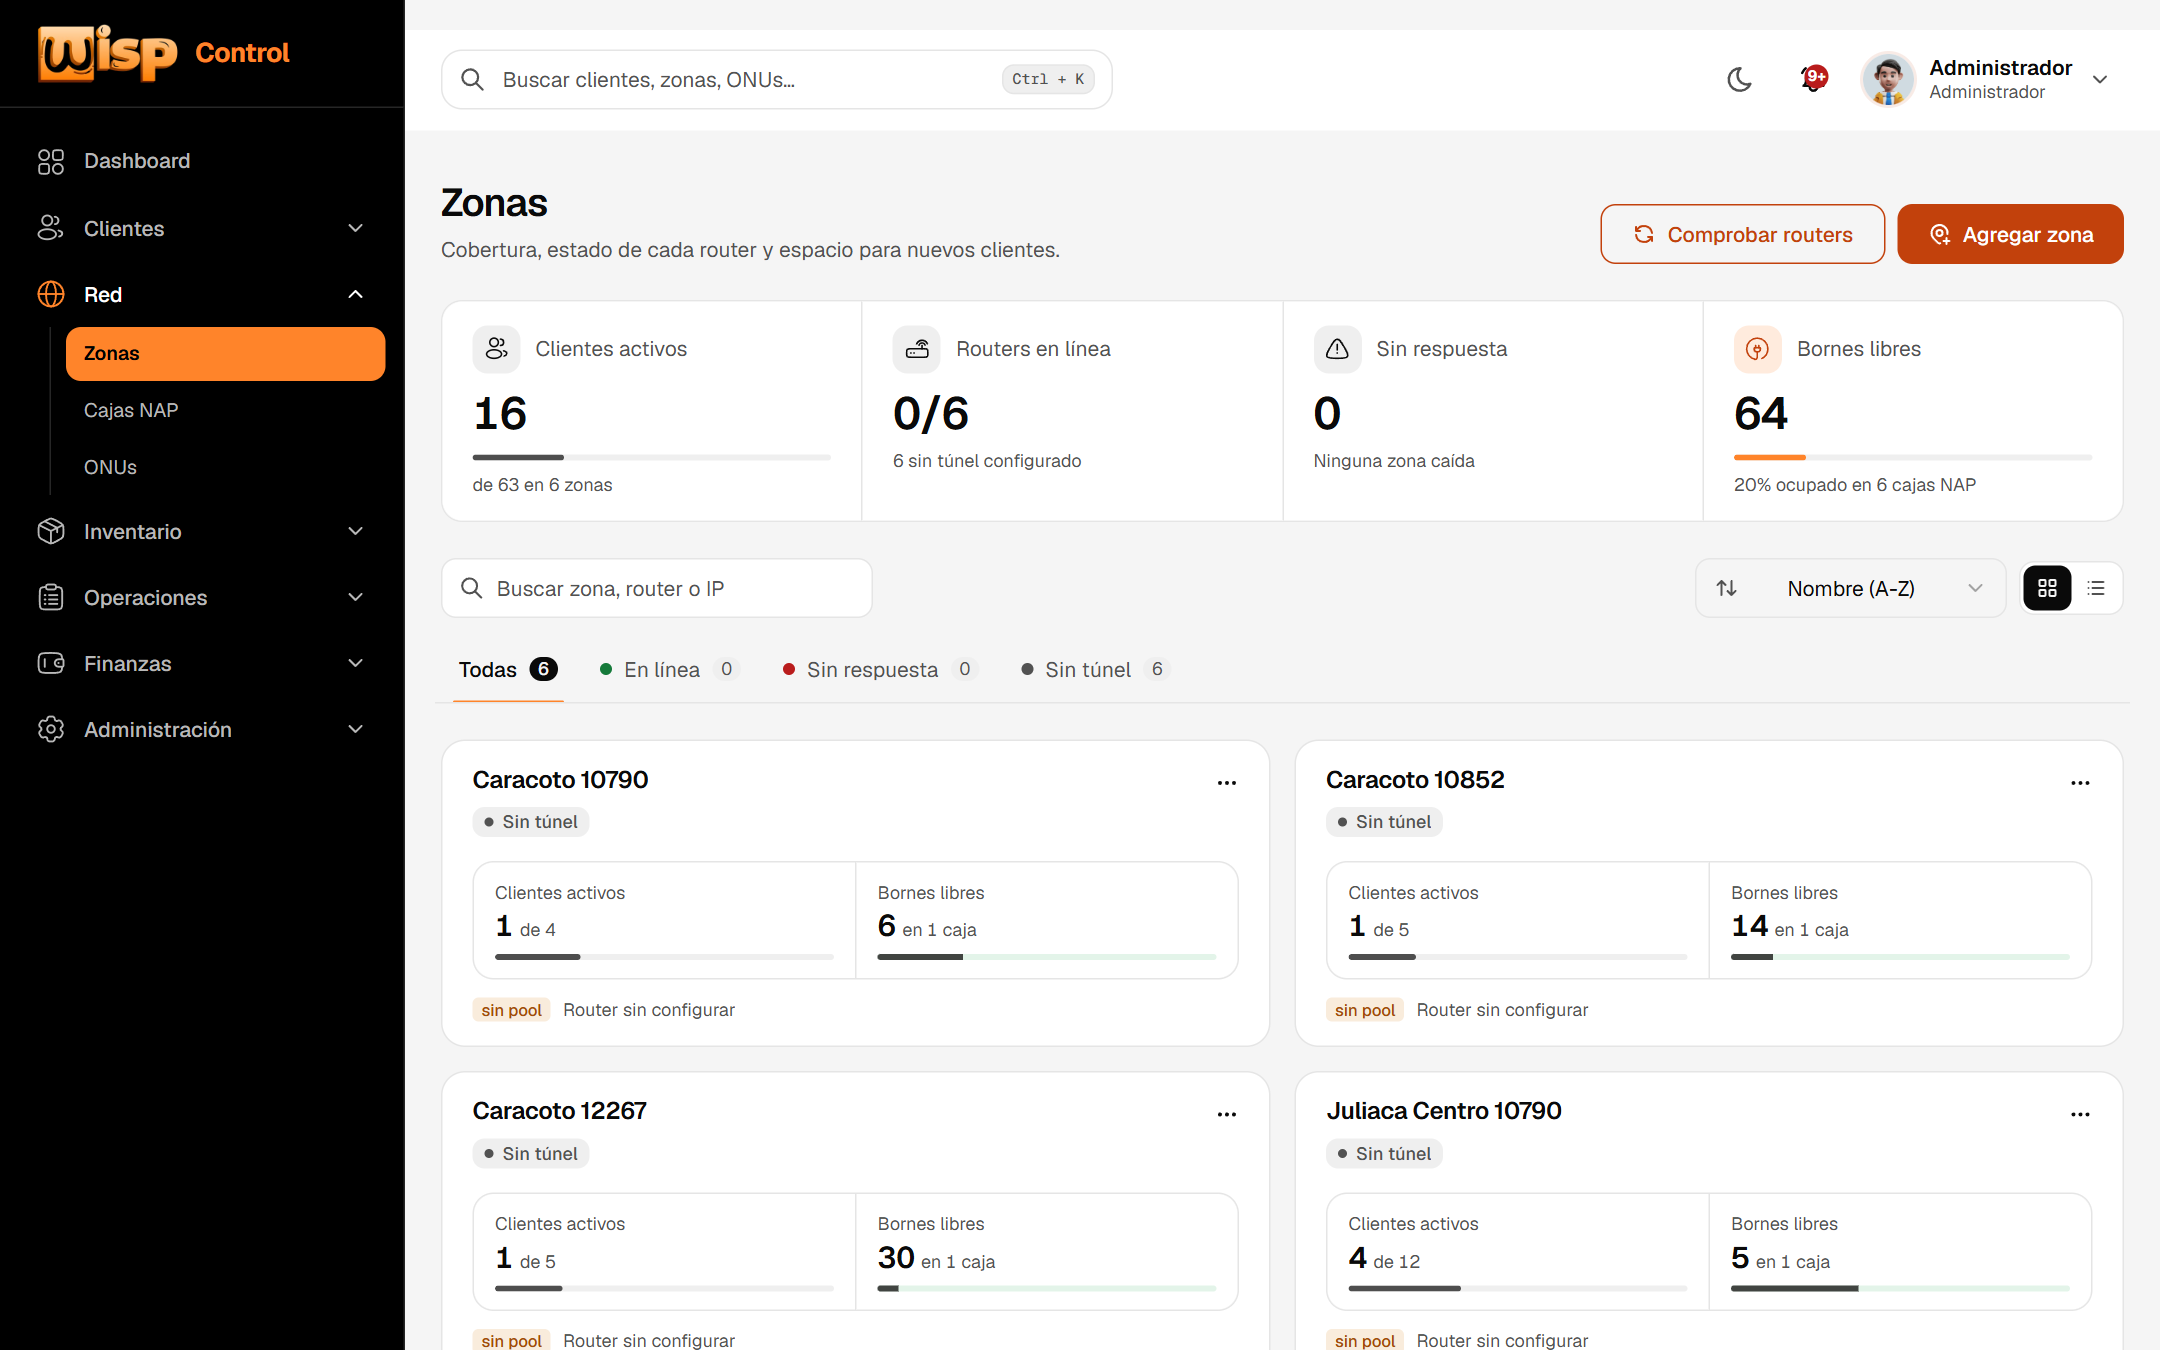
\includegraphics[width=\textwidth]{linea2/panel/p04_zonas.png}
\caption{Zonas: clientes activos, estado de los routers y del túnel WireGuard, y bornes libres por zona.}
\label{fig:ce02-e3-zonas}
\end{figure}

\begin{figure}[H]
\centering
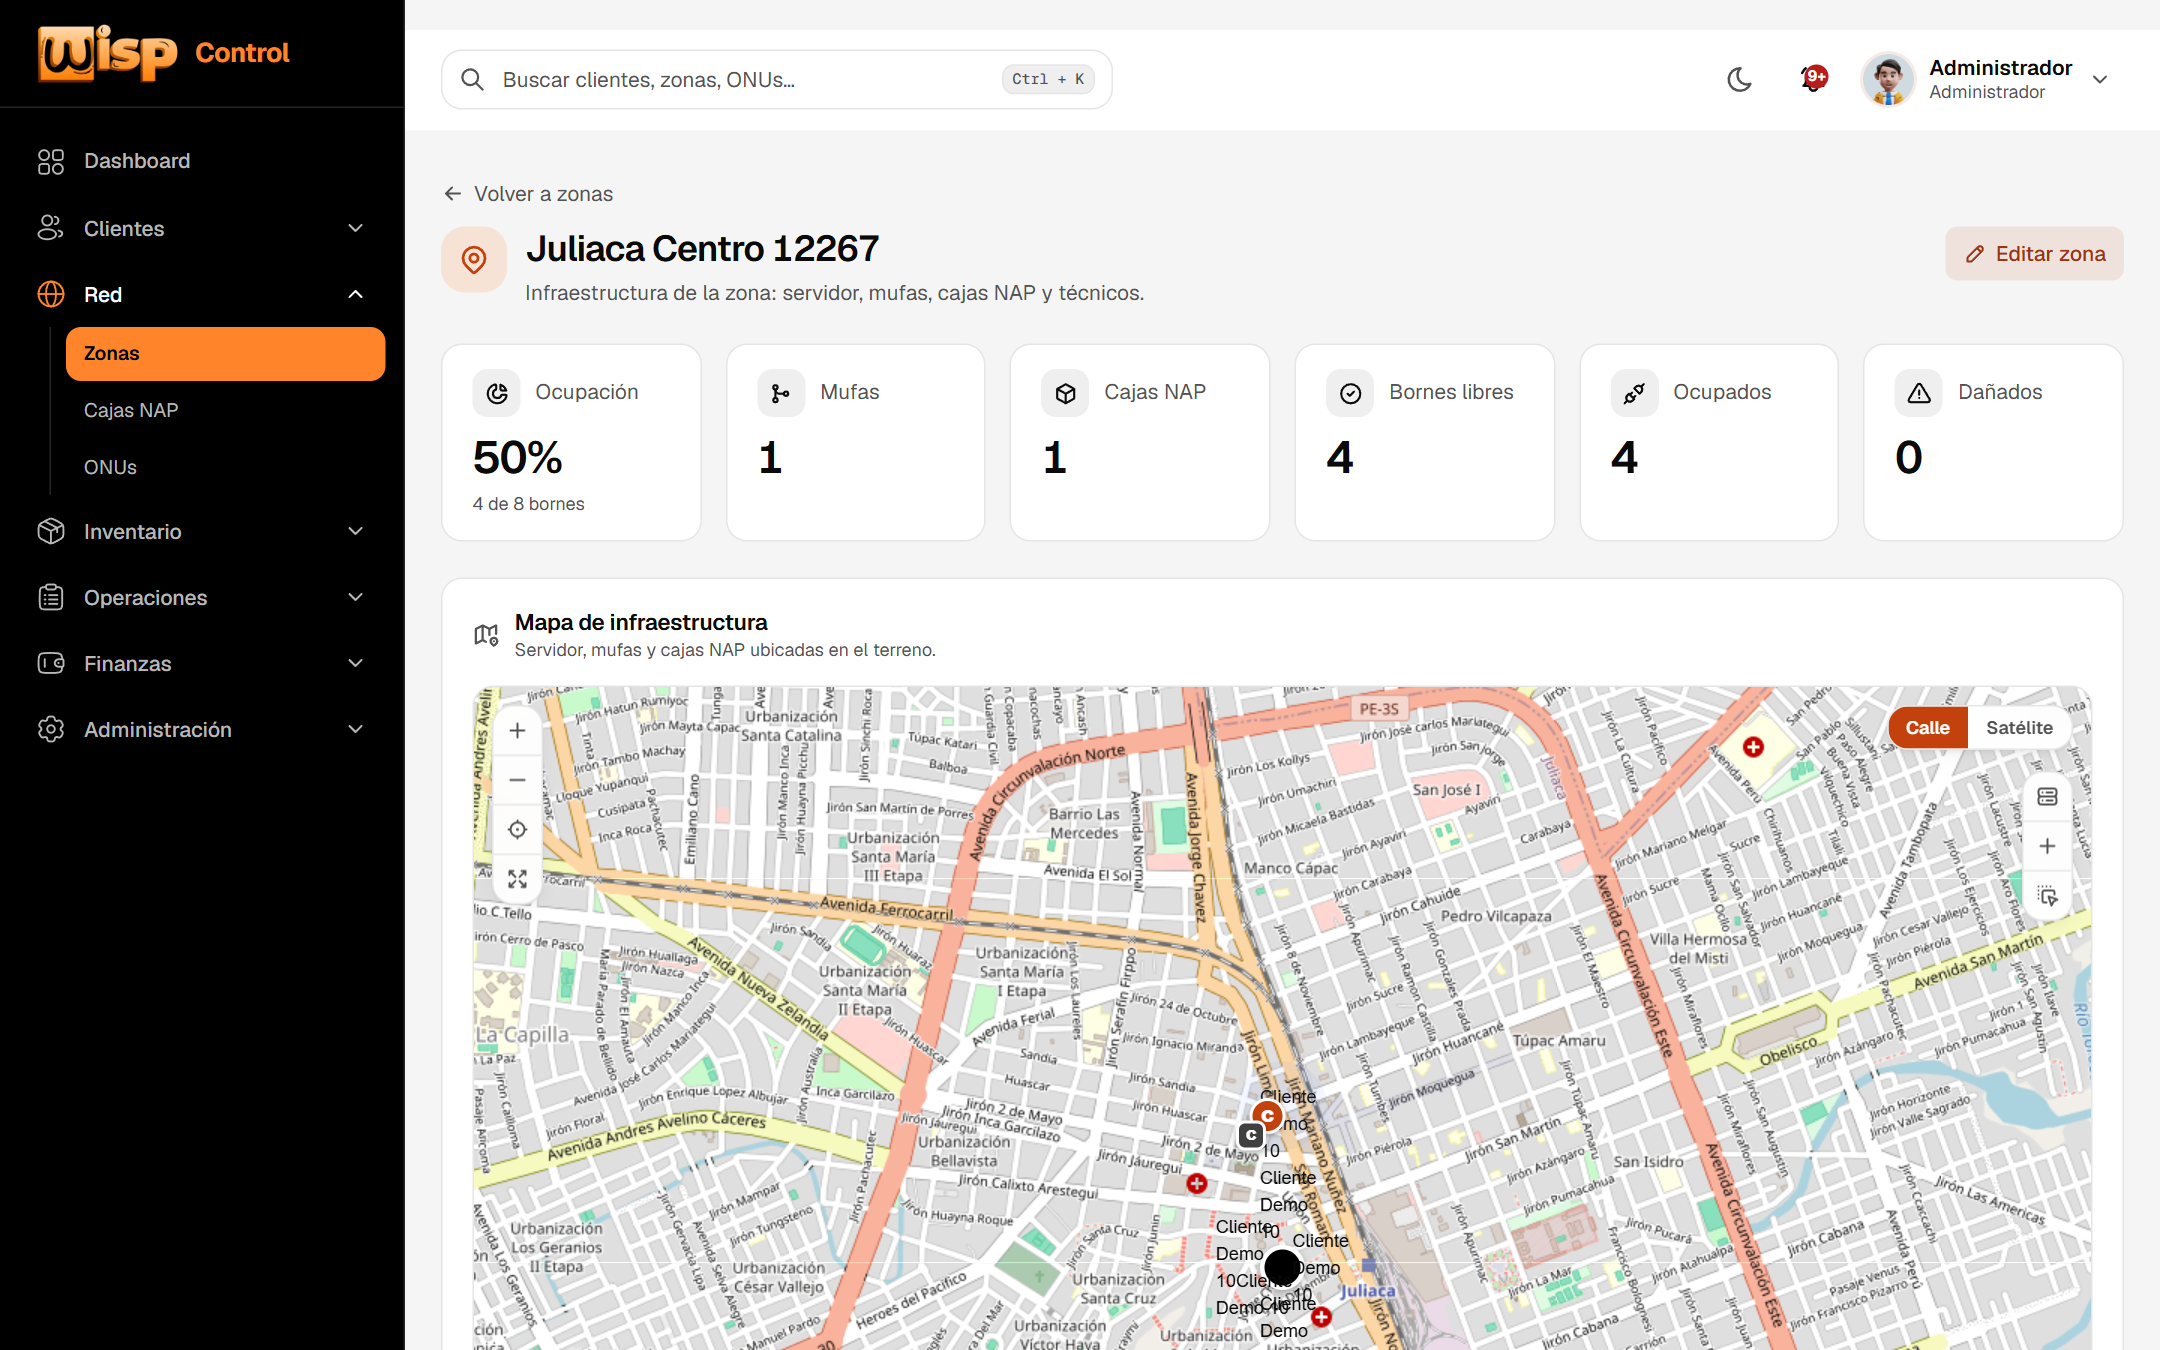
\includegraphics[width=\textwidth]{linea2/panel/p05_zona_detalle.png}
\caption{Detalle de una zona: ocupación de bornes y mapa de la infraestructura (mufas y cajas NAP).}
\label{fig:ce02-e3-zona-detalle}
\end{figure}

\begin{figure}[H]
\centering
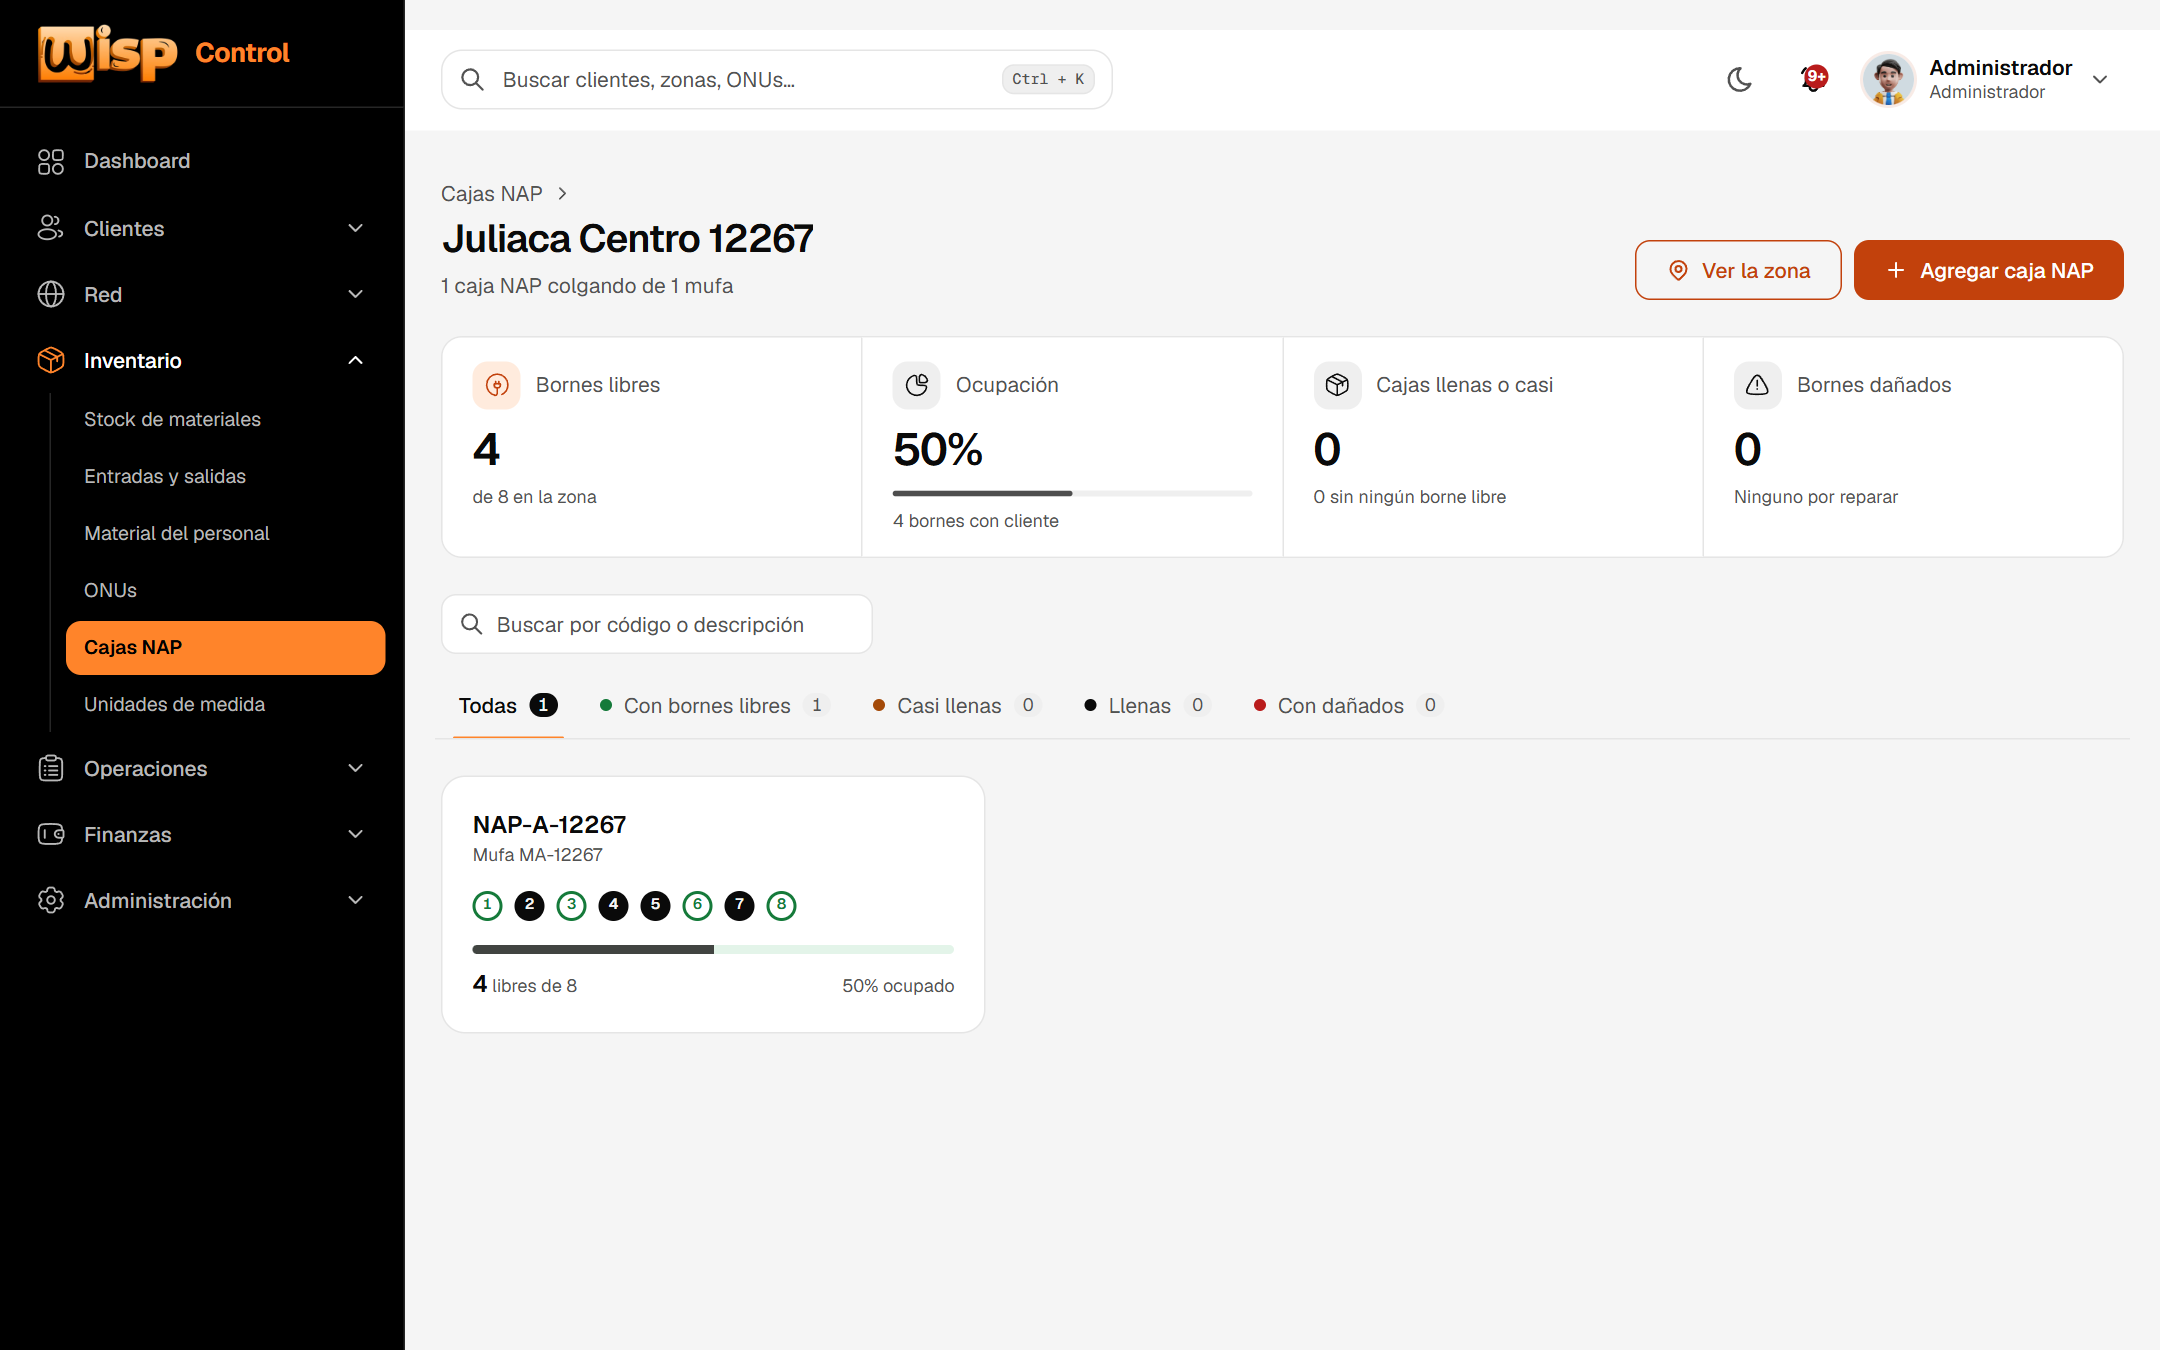
\includegraphics[width=\textwidth]{linea2/panel/p06_cajas_nap.png}
\caption{Cajas NAP de una zona con el estado de cada borne (libre, ocupado, dañado).}
\label{fig:ce02-e3-cajas-nap}
\end{figure}

\begin{figure}[H]
\centering
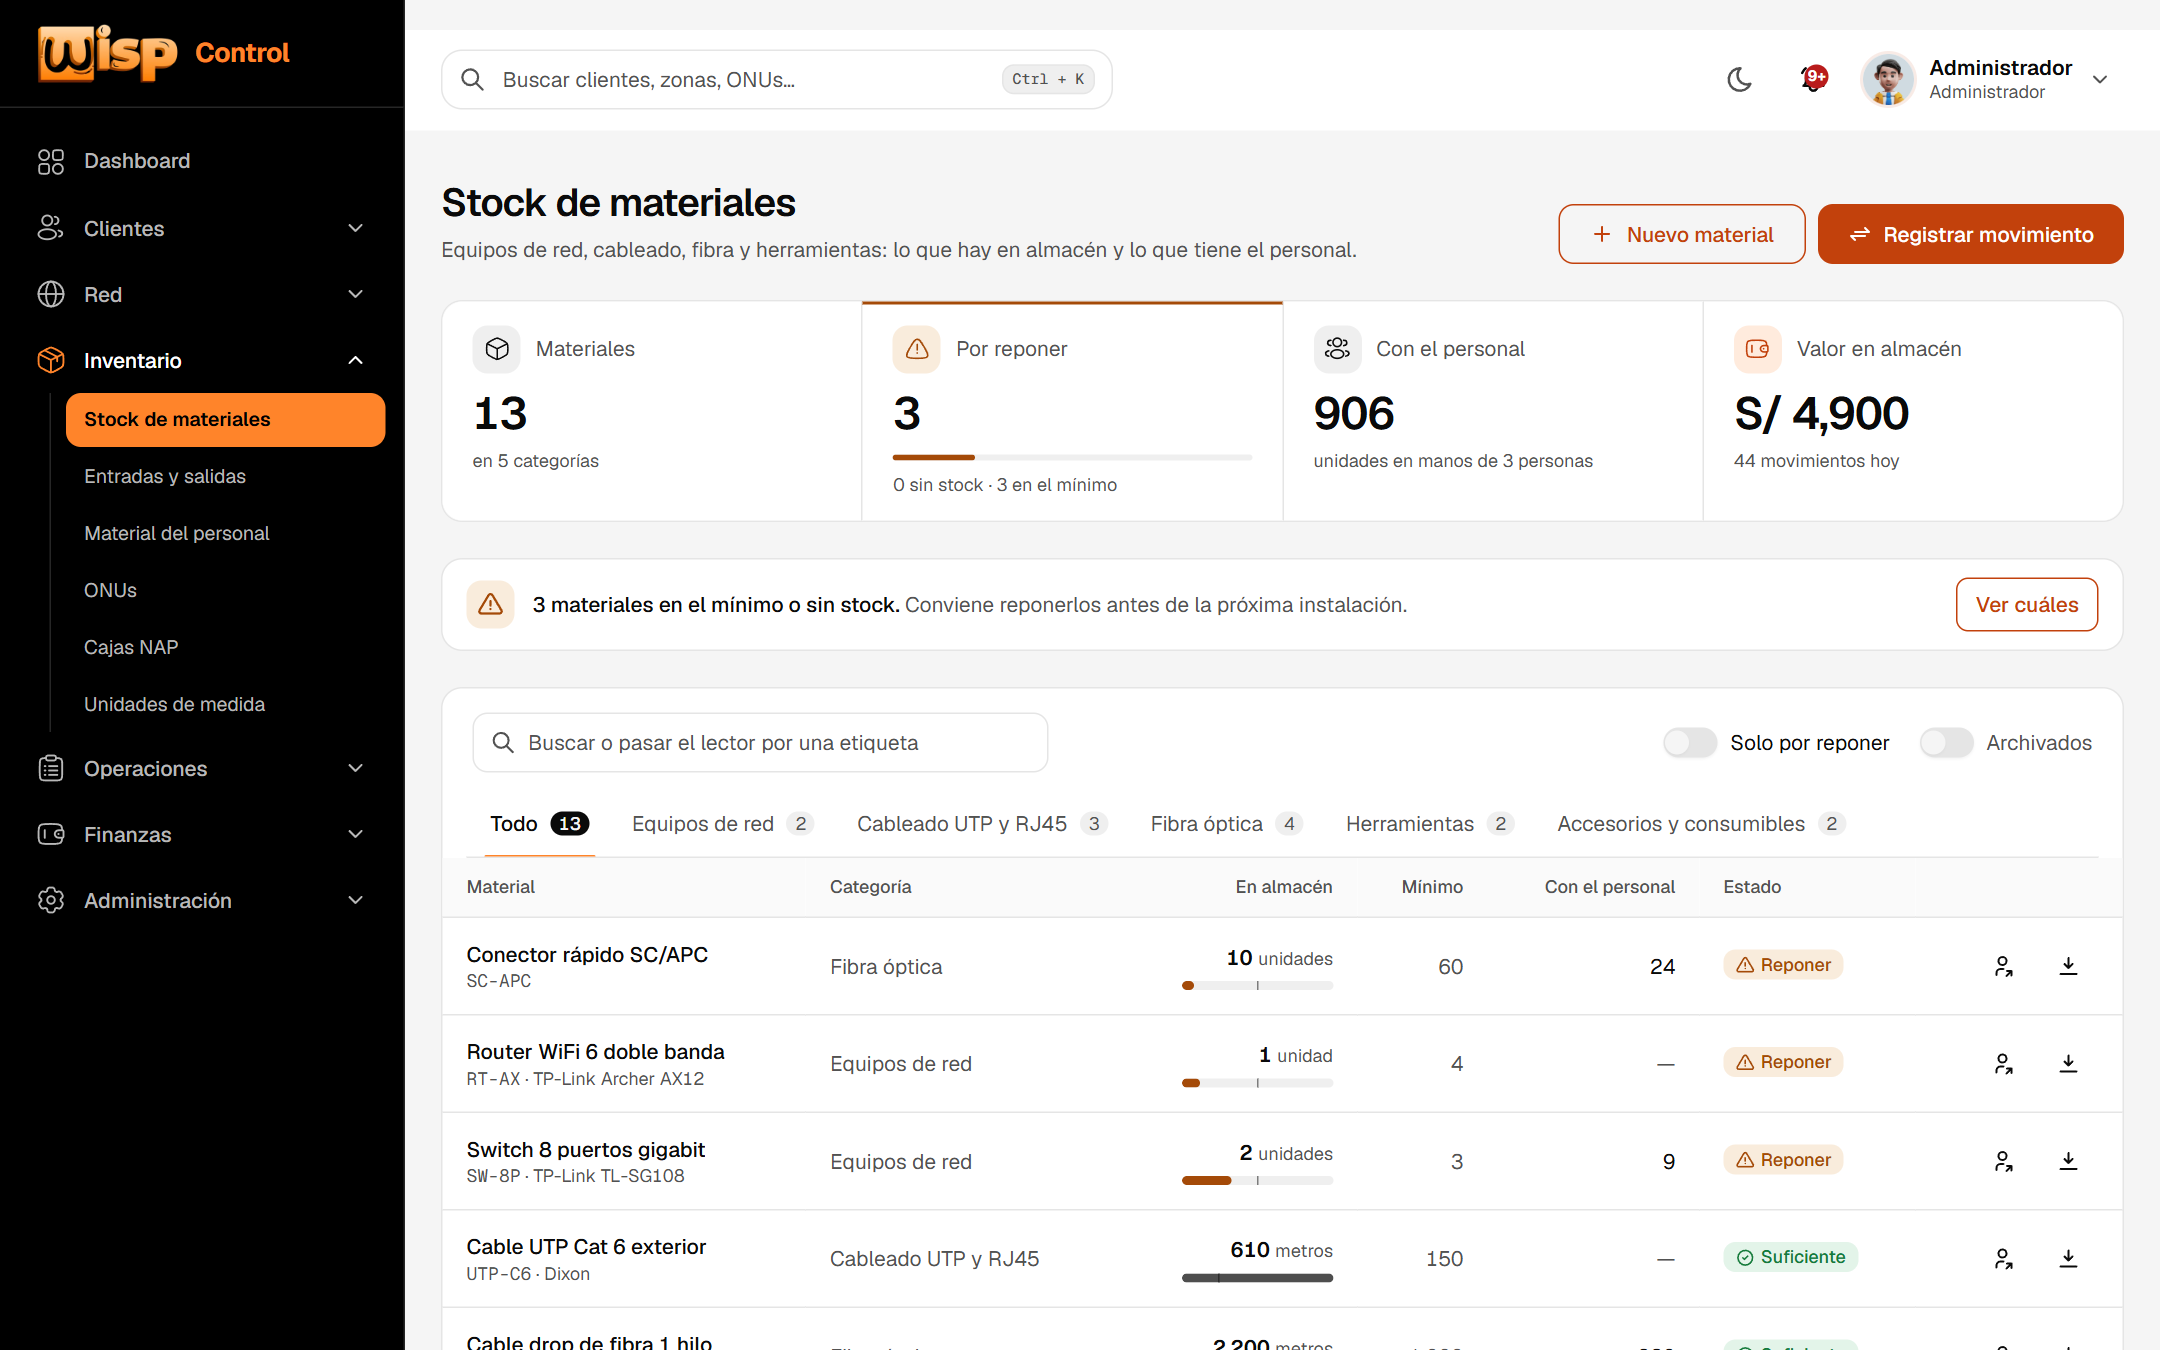
\includegraphics[width=\textwidth]{linea2/panel/p07_inventario.png}
\caption{Stock de materiales: existencias en almacén y en manos del personal, alertas de reposición y movimientos.}
\label{fig:ce02-e3-inventario}
\end{figure}

\begin{figure}[H]
\centering
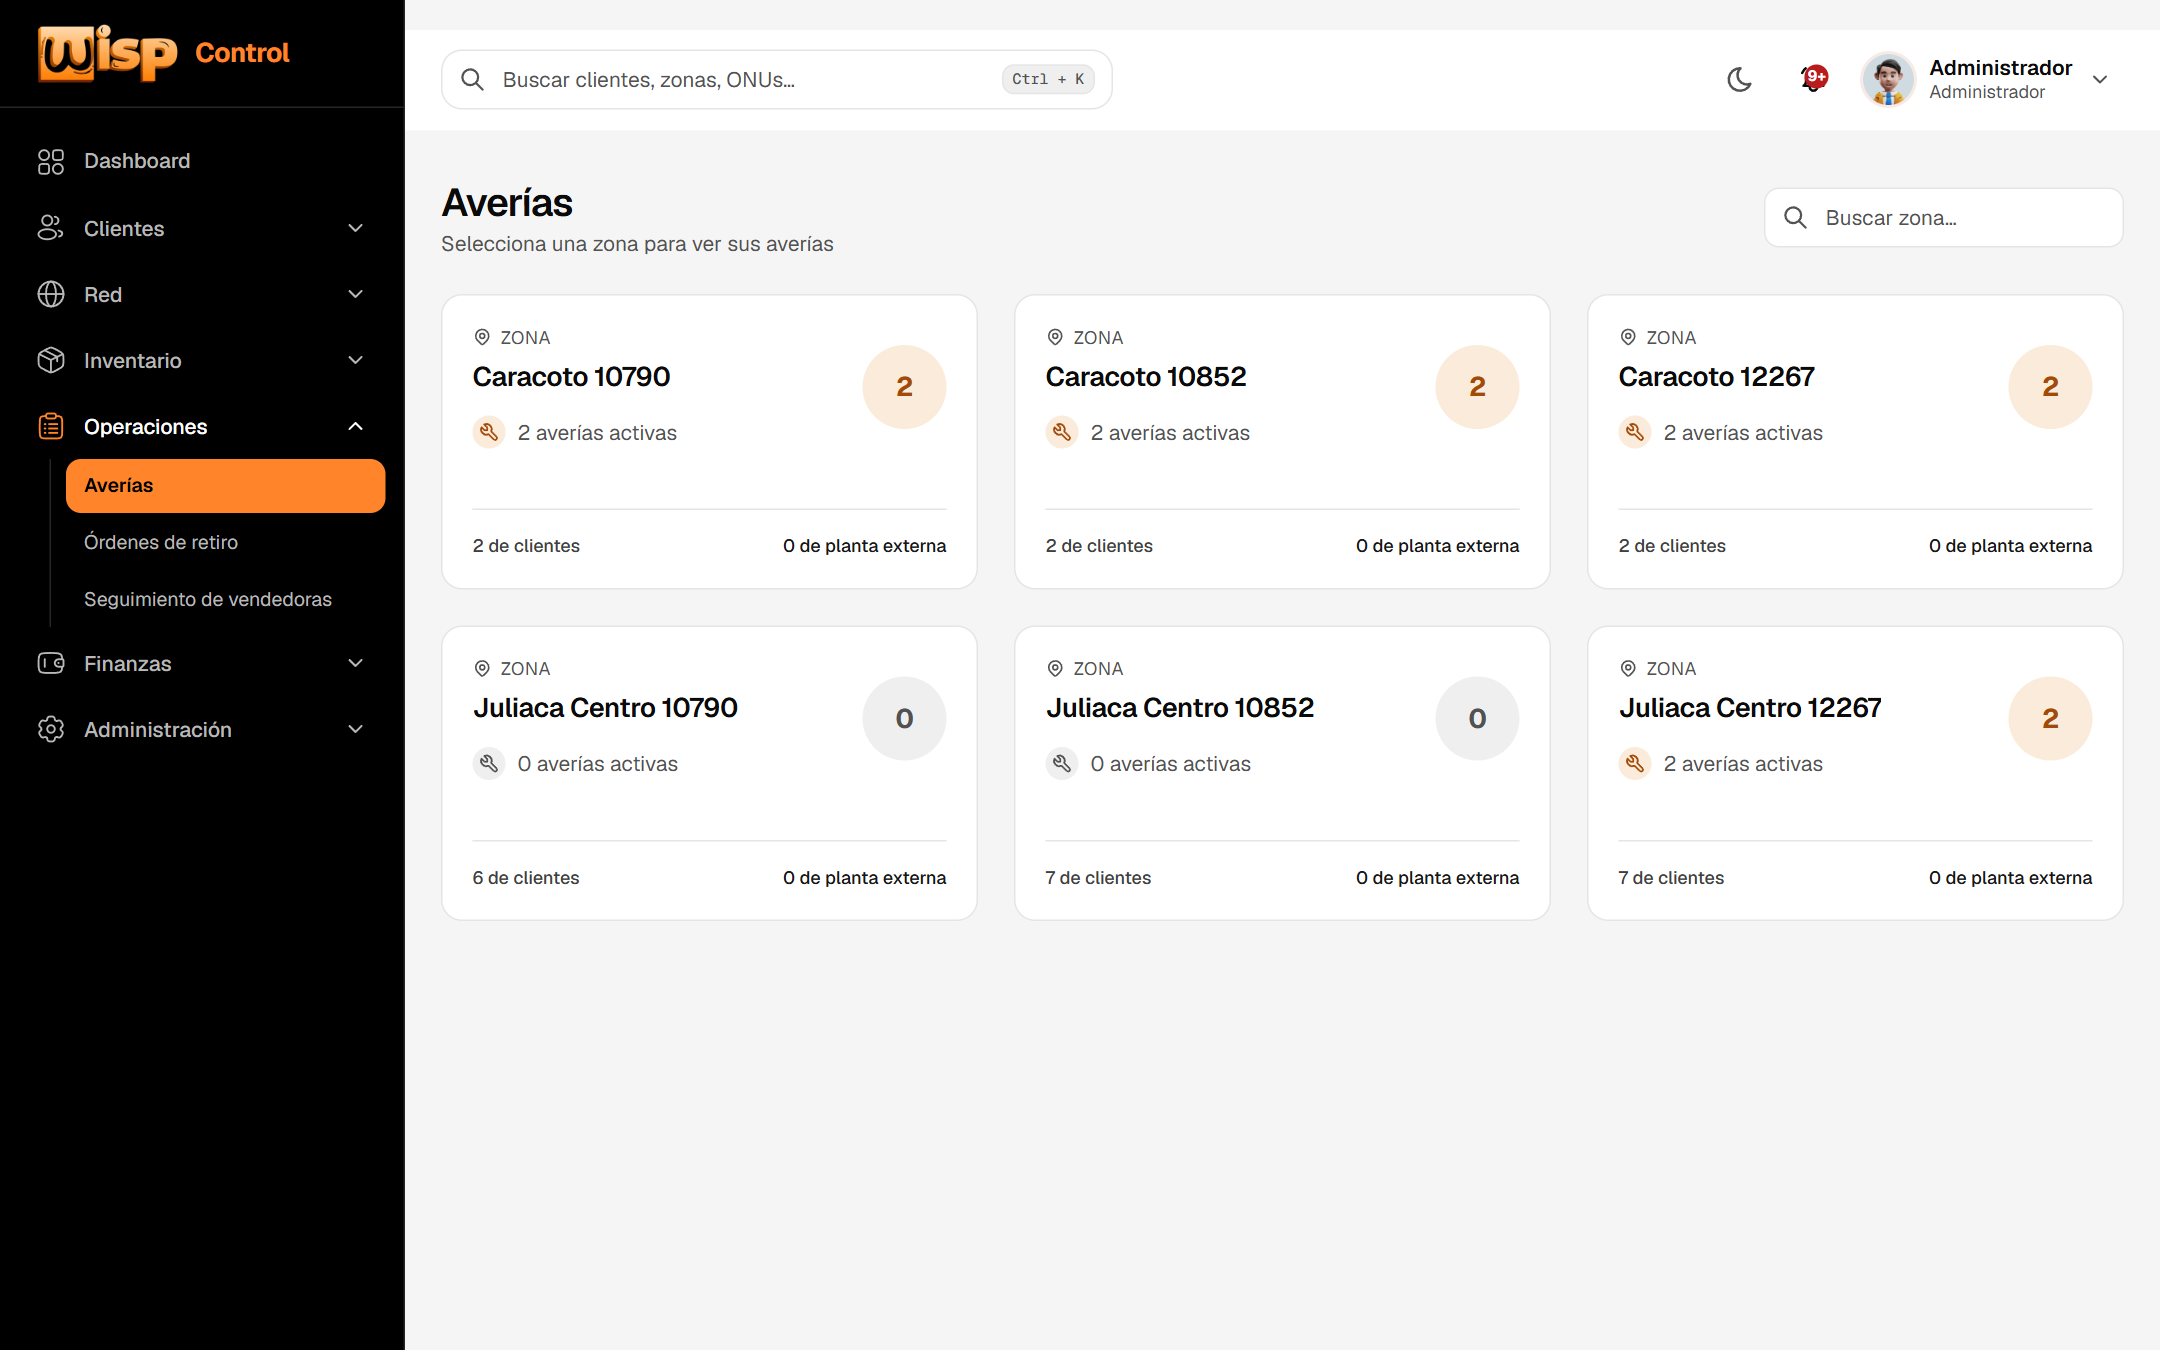
\includegraphics[width=\textwidth]{linea2/panel/p08_averias.png}
\caption{Averías agrupadas por zona para su asignación a los técnicos.}
\label{fig:ce02-e3-averias}
\end{figure}

\begin{figure}[H]
\centering
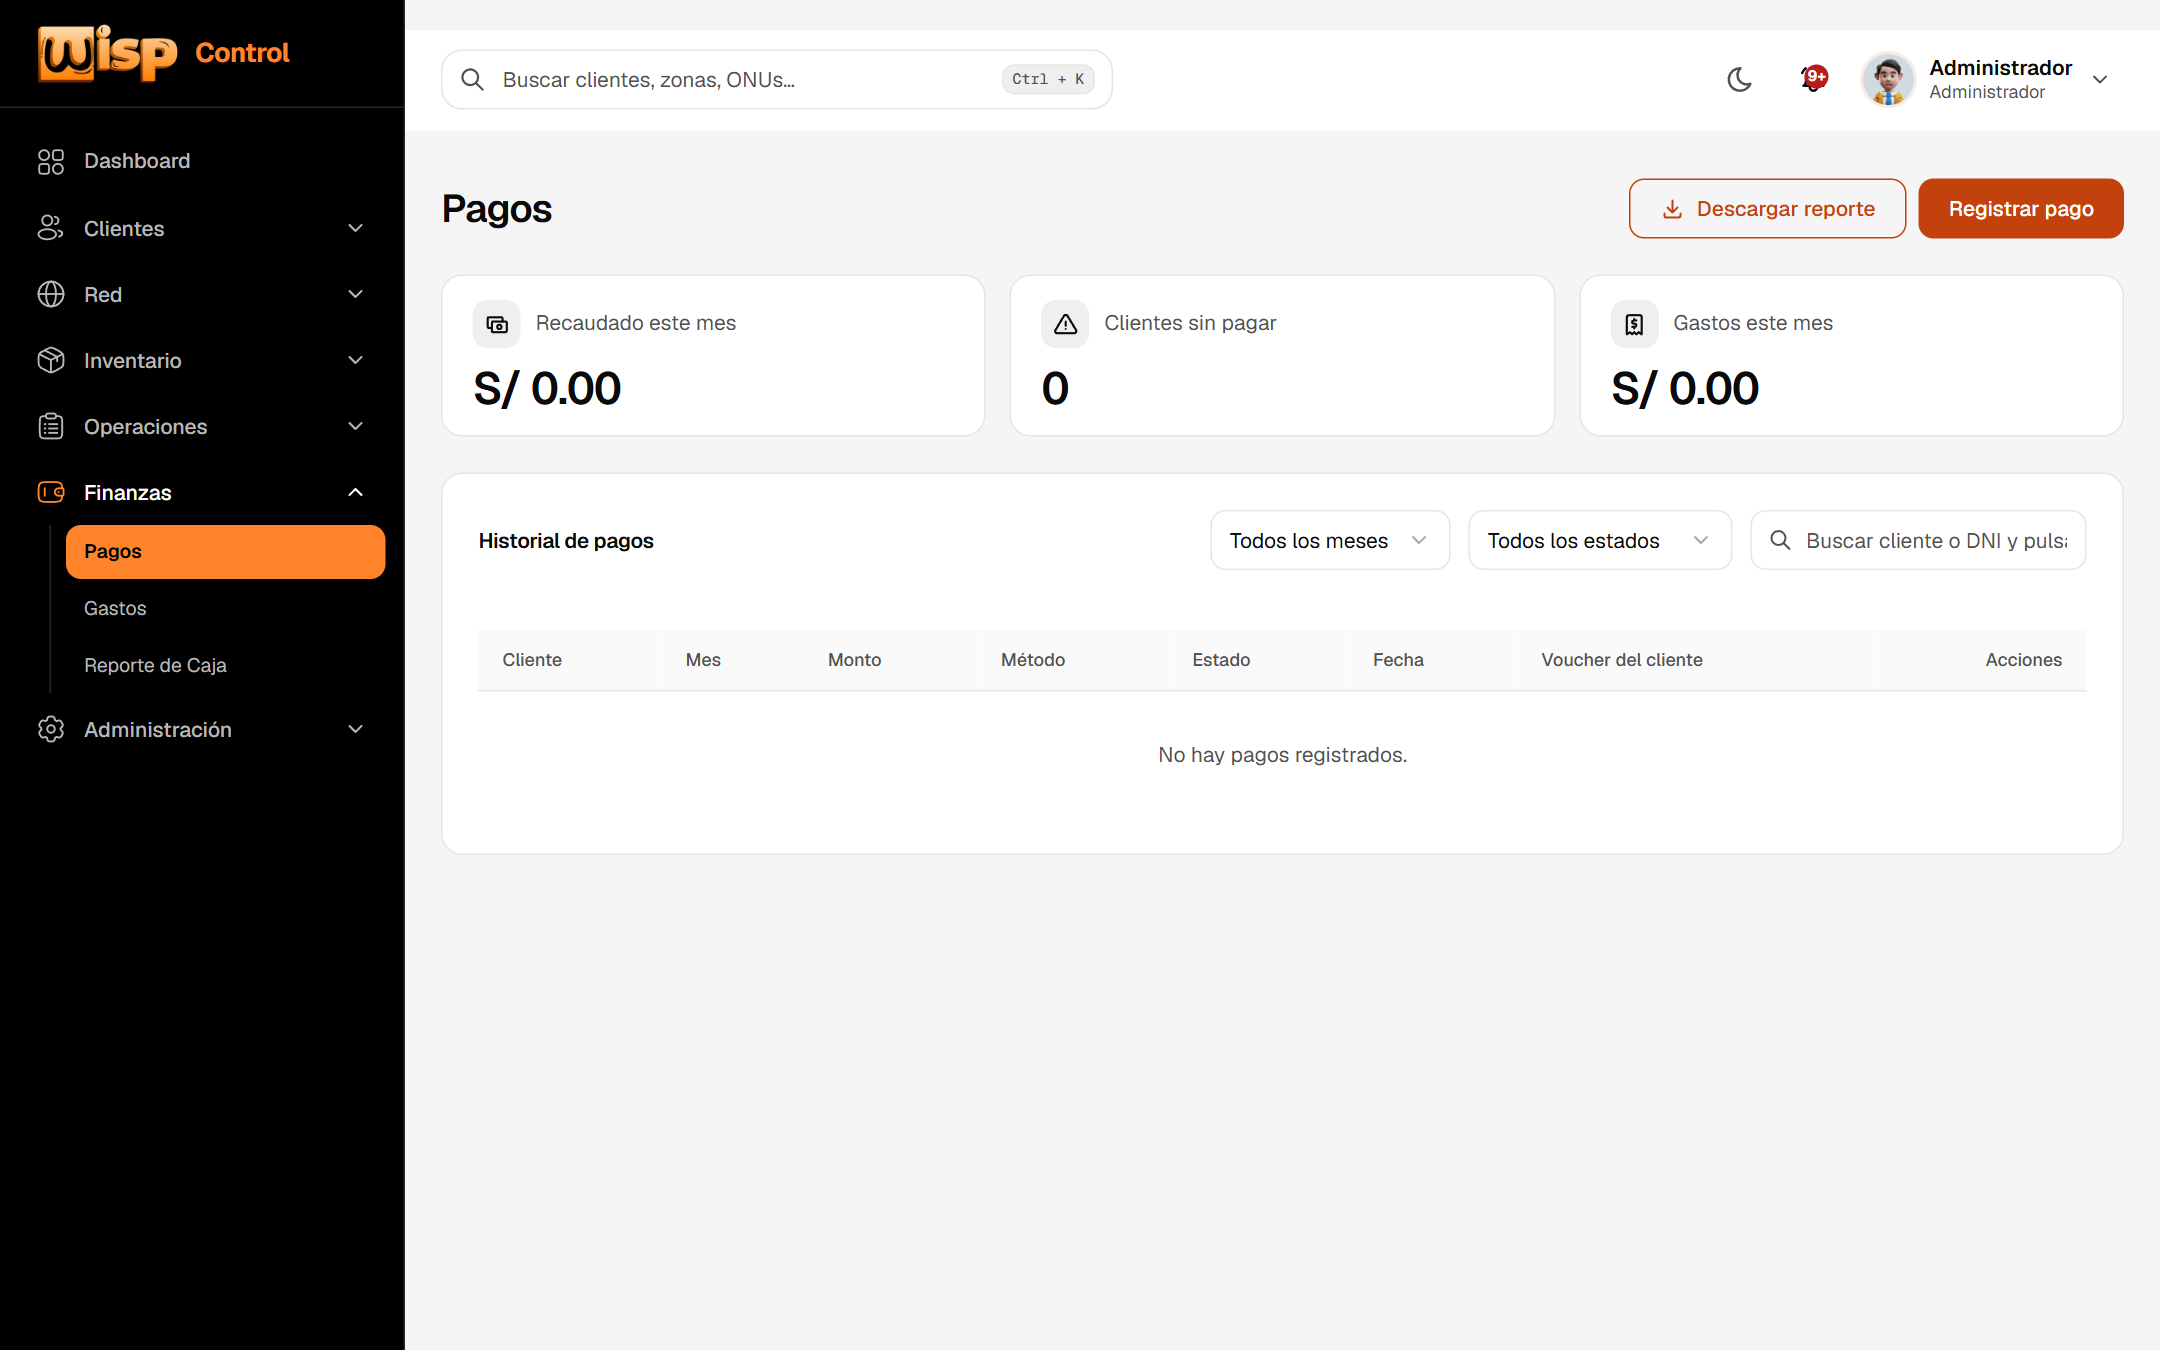
\includegraphics[width=\textwidth]{linea2/panel/p09_pagos.png}
\caption{Pagos: recaudación del mes, clientes sin pagar e historial con filtros.}
\label{fig:ce02-e3-pagos}
\end{figure}

\begin{figure}[H]
\centering
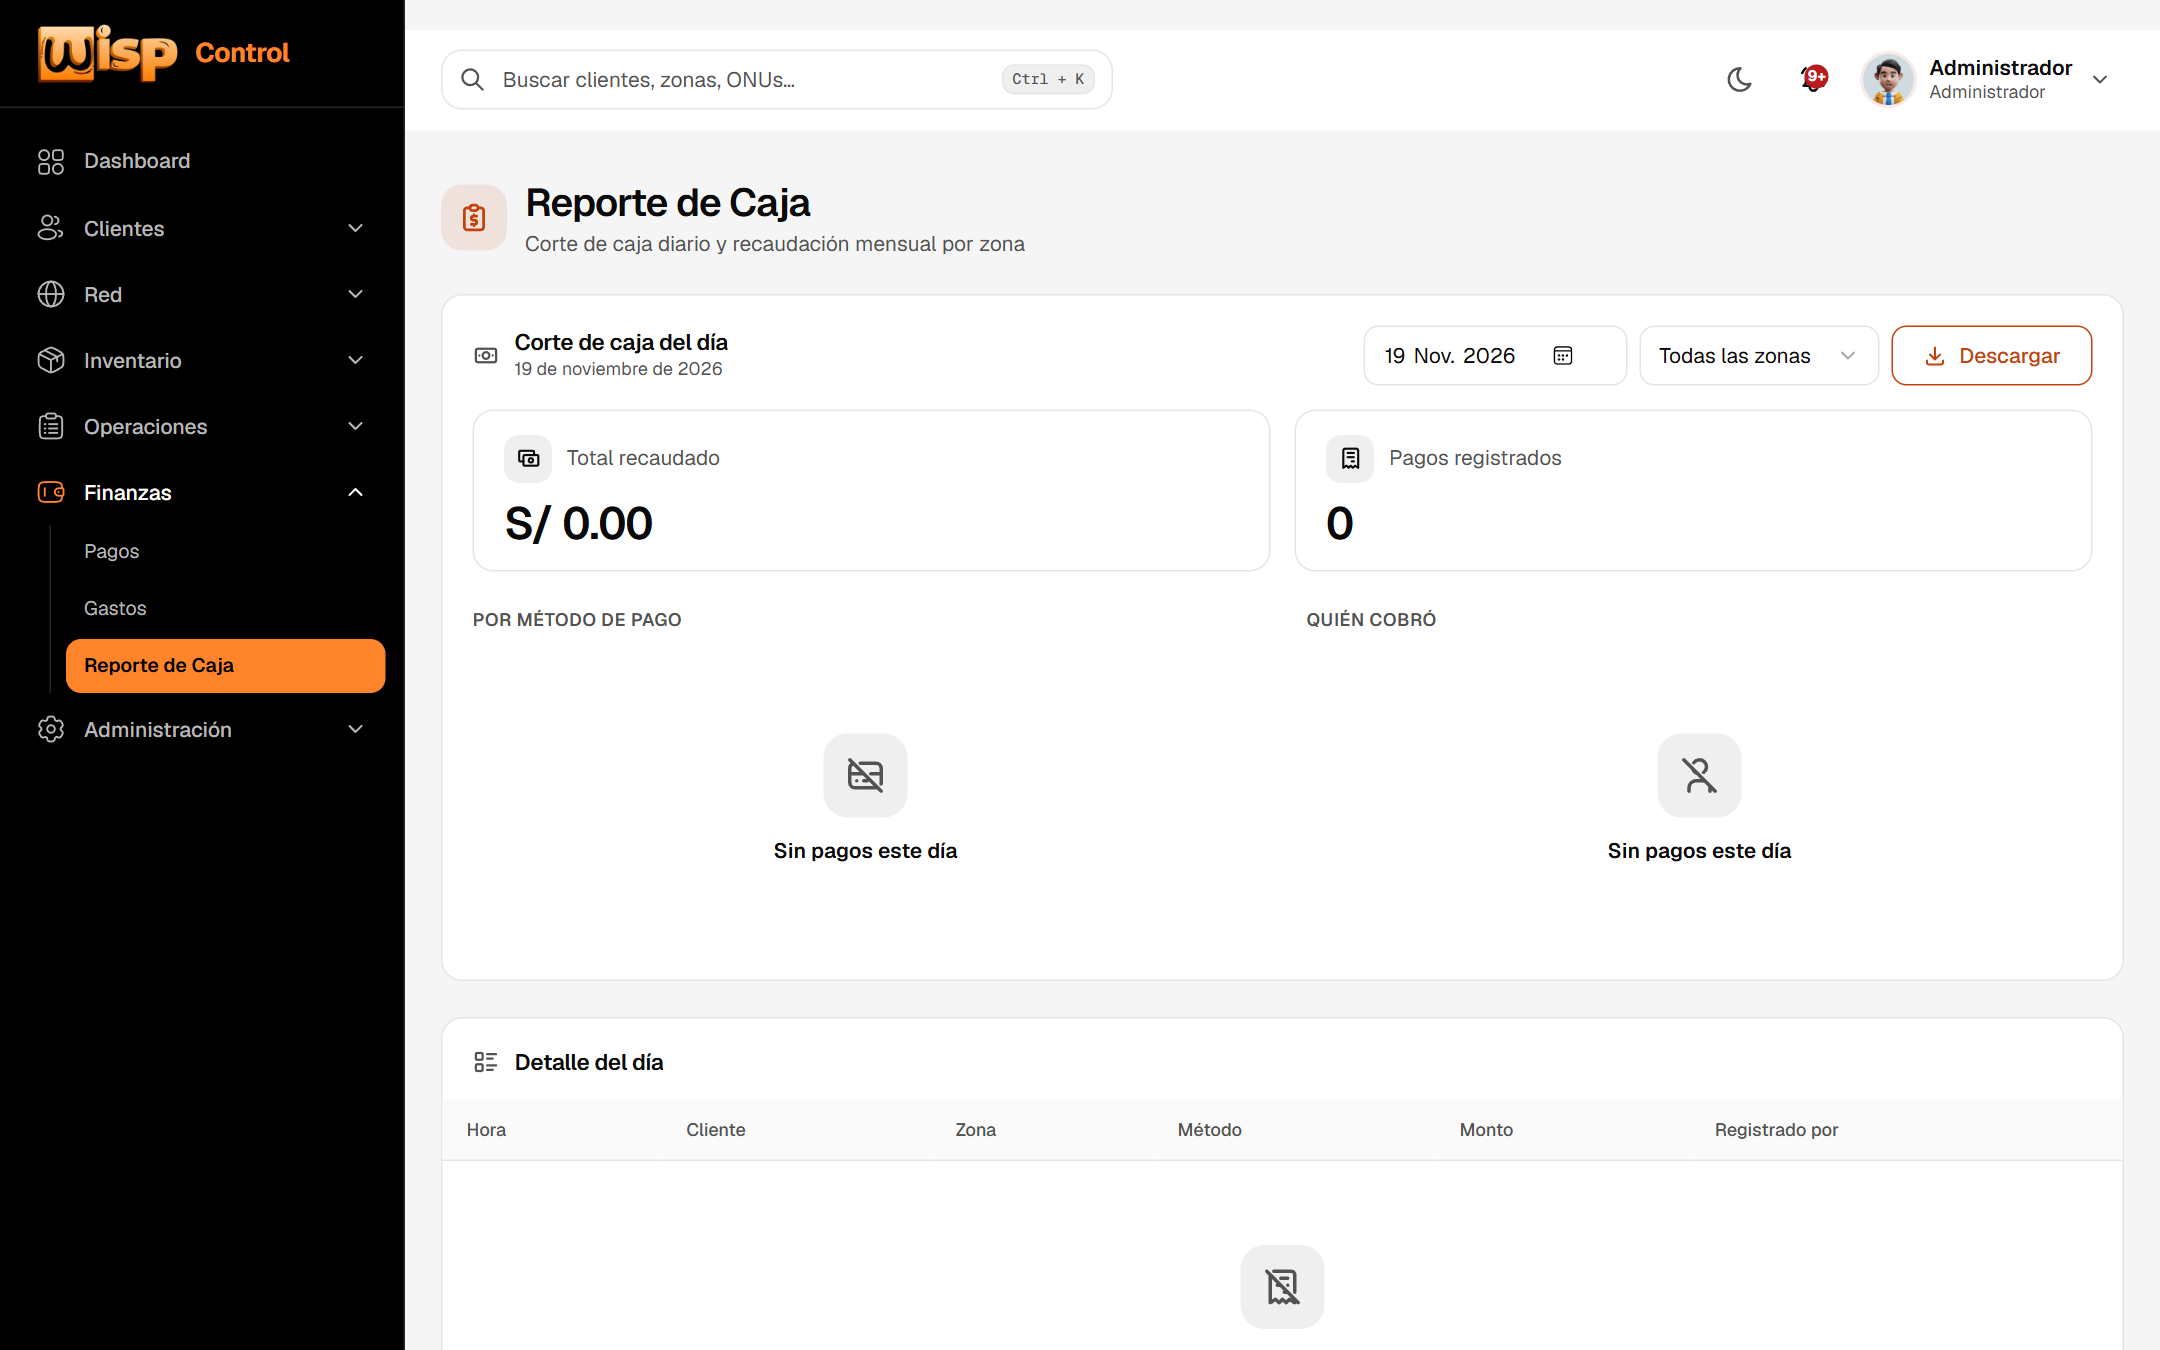
\includegraphics[width=\textwidth]{linea2/panel/p13_reporte_caja.png}
\caption{Reporte de caja diario: total recaudado por método de pago y por quién cobró.}
\label{fig:ce02-e3-reporte-caja}
\end{figure}

\begin{figure}[H]
\centering
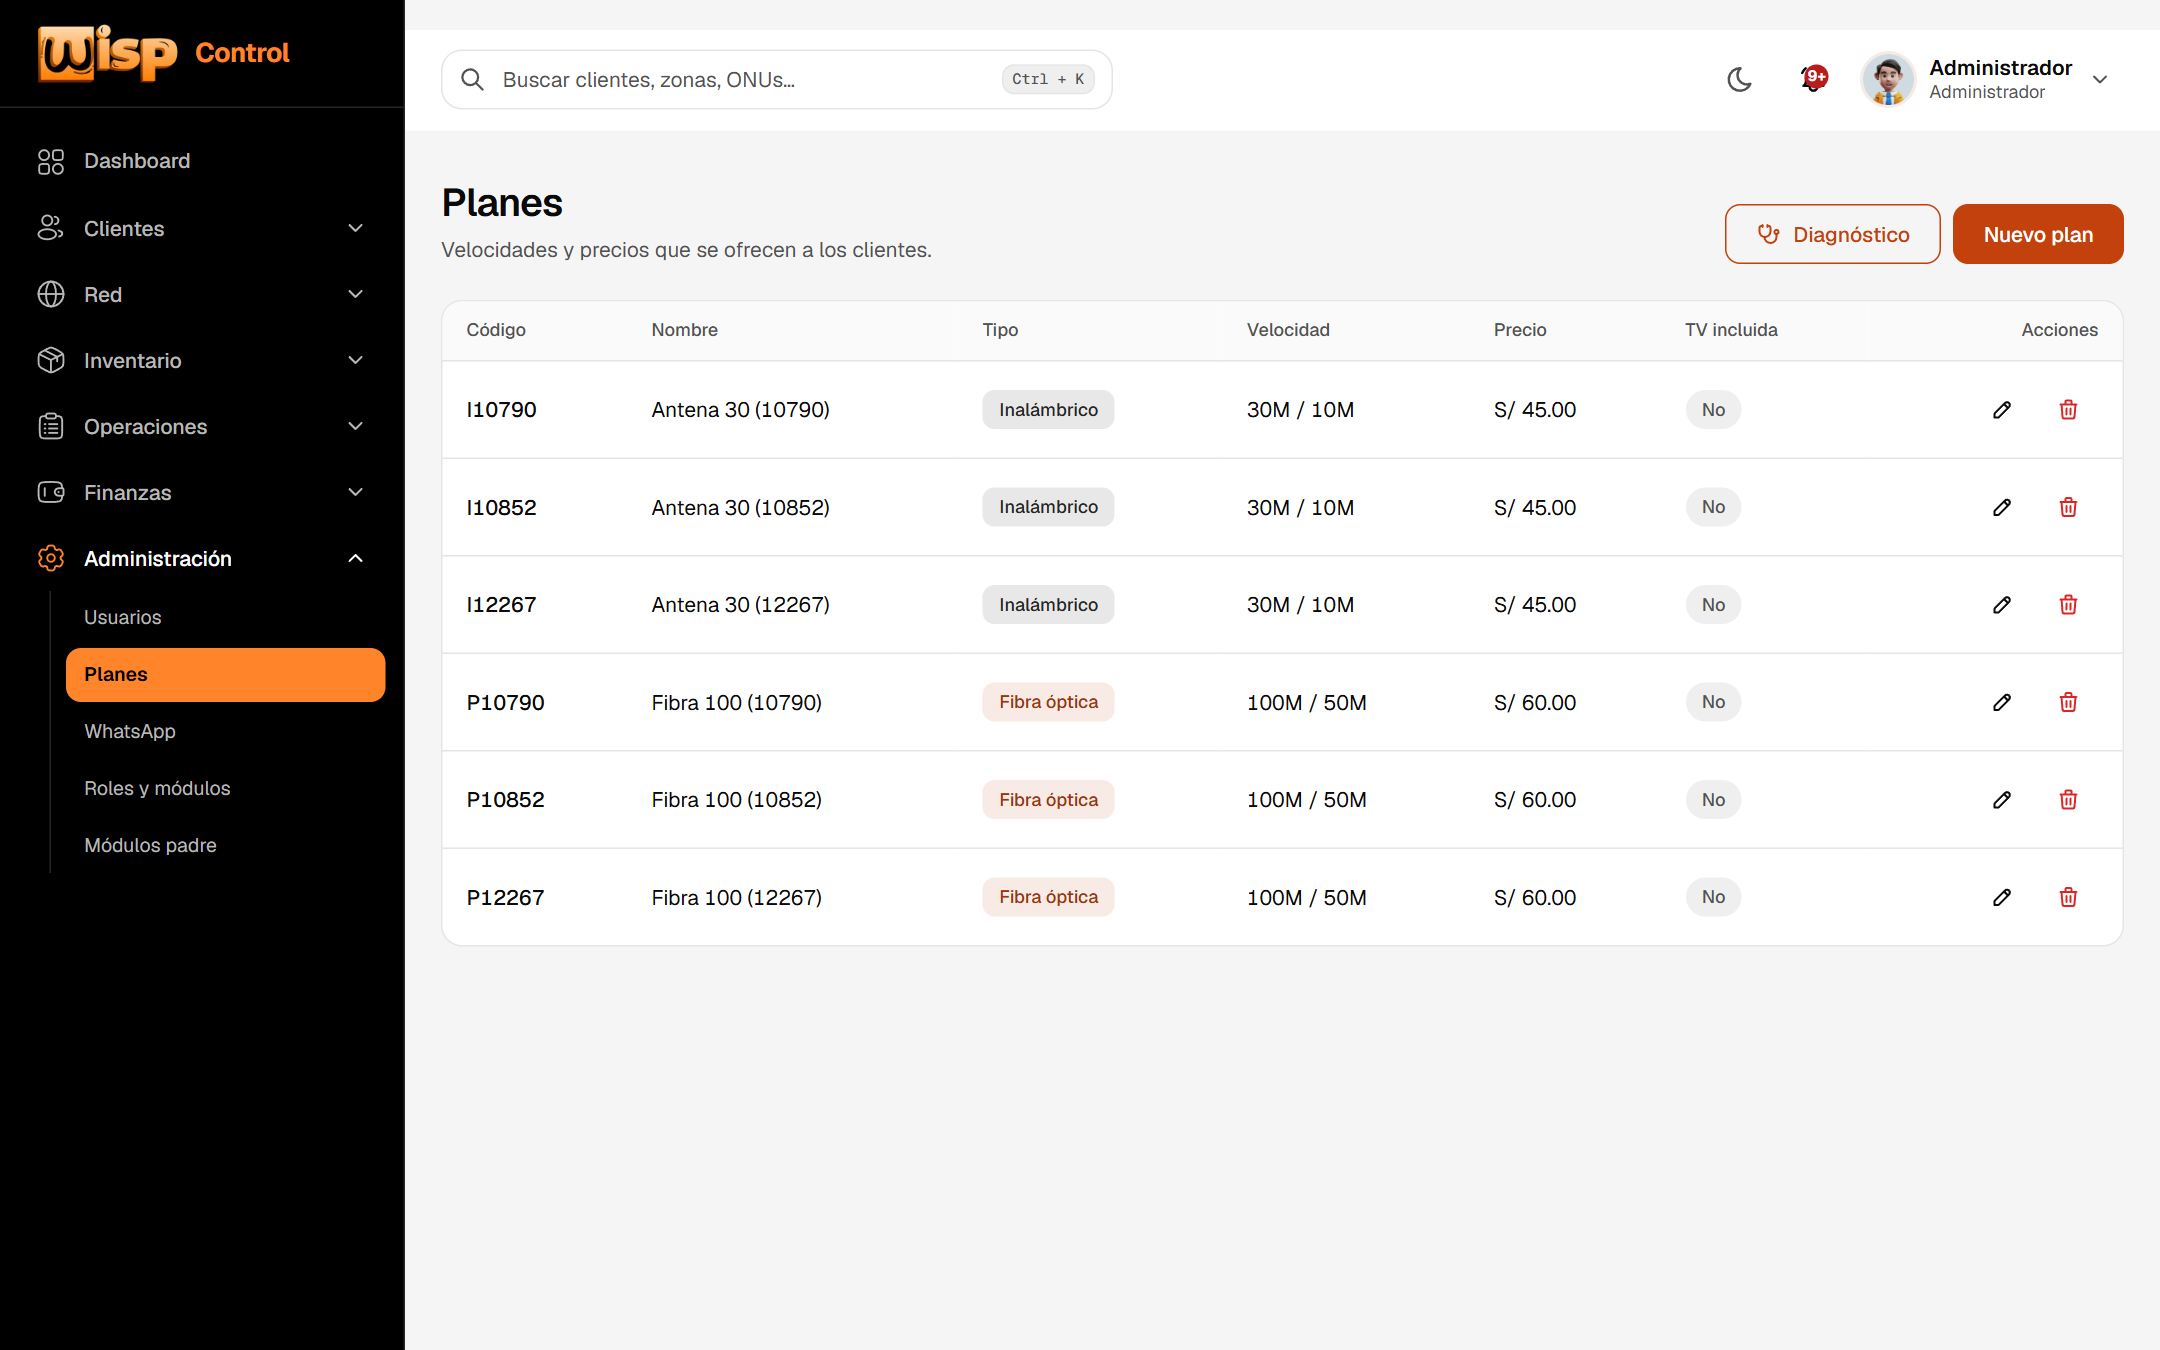
\includegraphics[width=\textwidth]{linea2/panel/p10_planes.png}
\caption{Catálogo de planes con velocidad, precio y tipo de conexión.}
\label{fig:ce02-e3-planes}
\end{figure}

\begin{figure}[H]
\centering
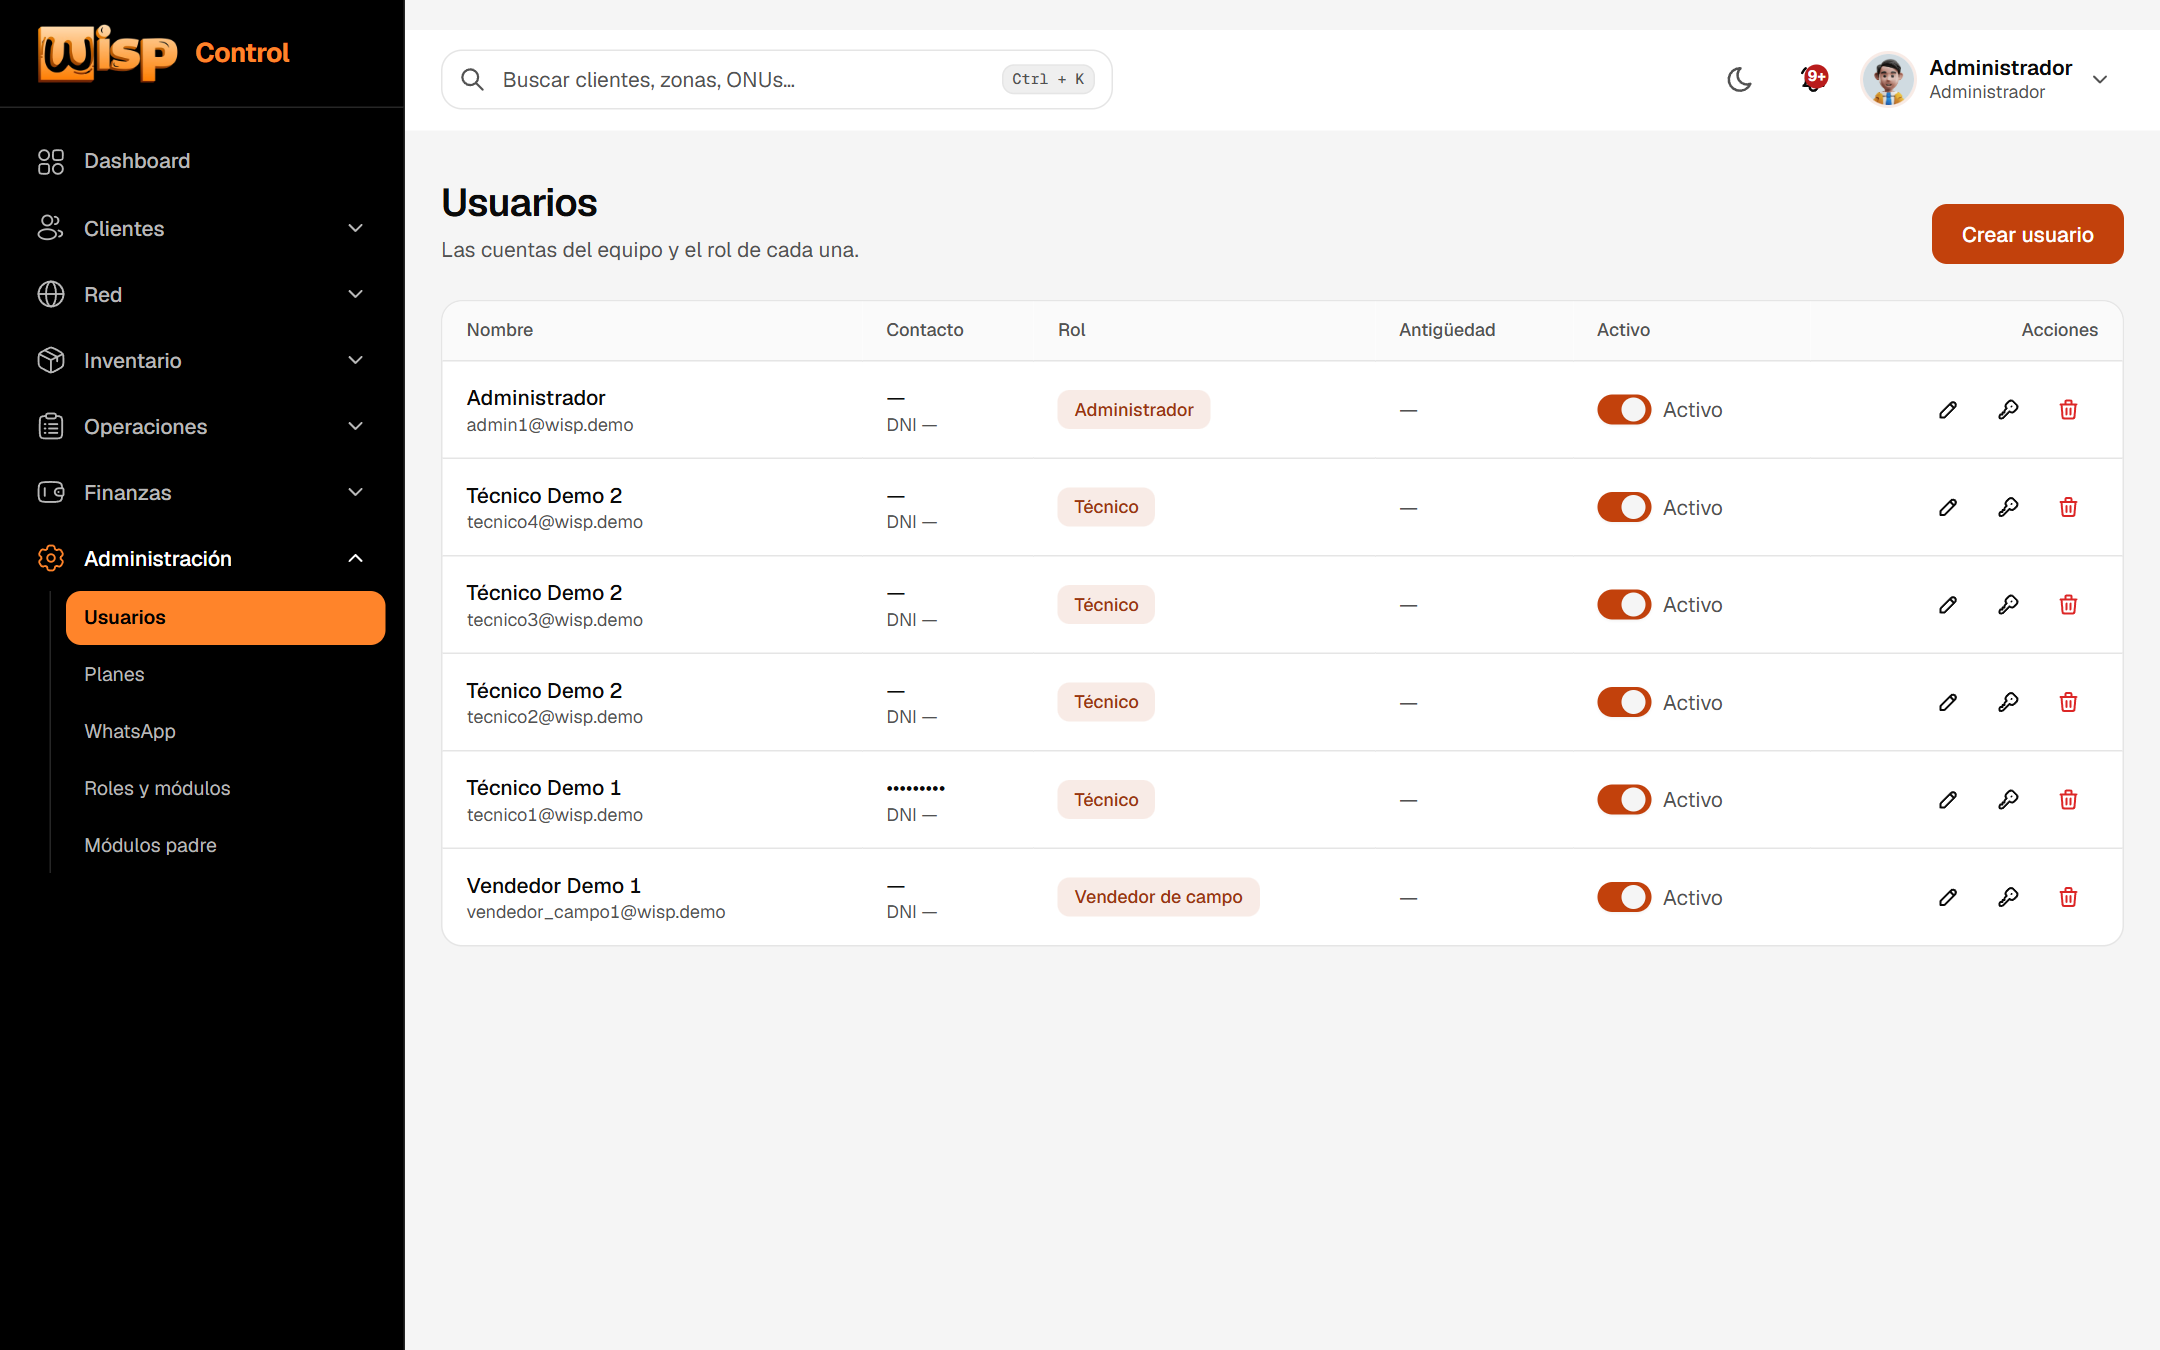
\includegraphics[width=\textwidth]{linea2/panel/p11_usuarios.png}
\caption{Usuarios del equipo con su rol y estado.}
\label{fig:ce02-e3-usuarios}
\end{figure}

\begin{figure}[H]
\centering
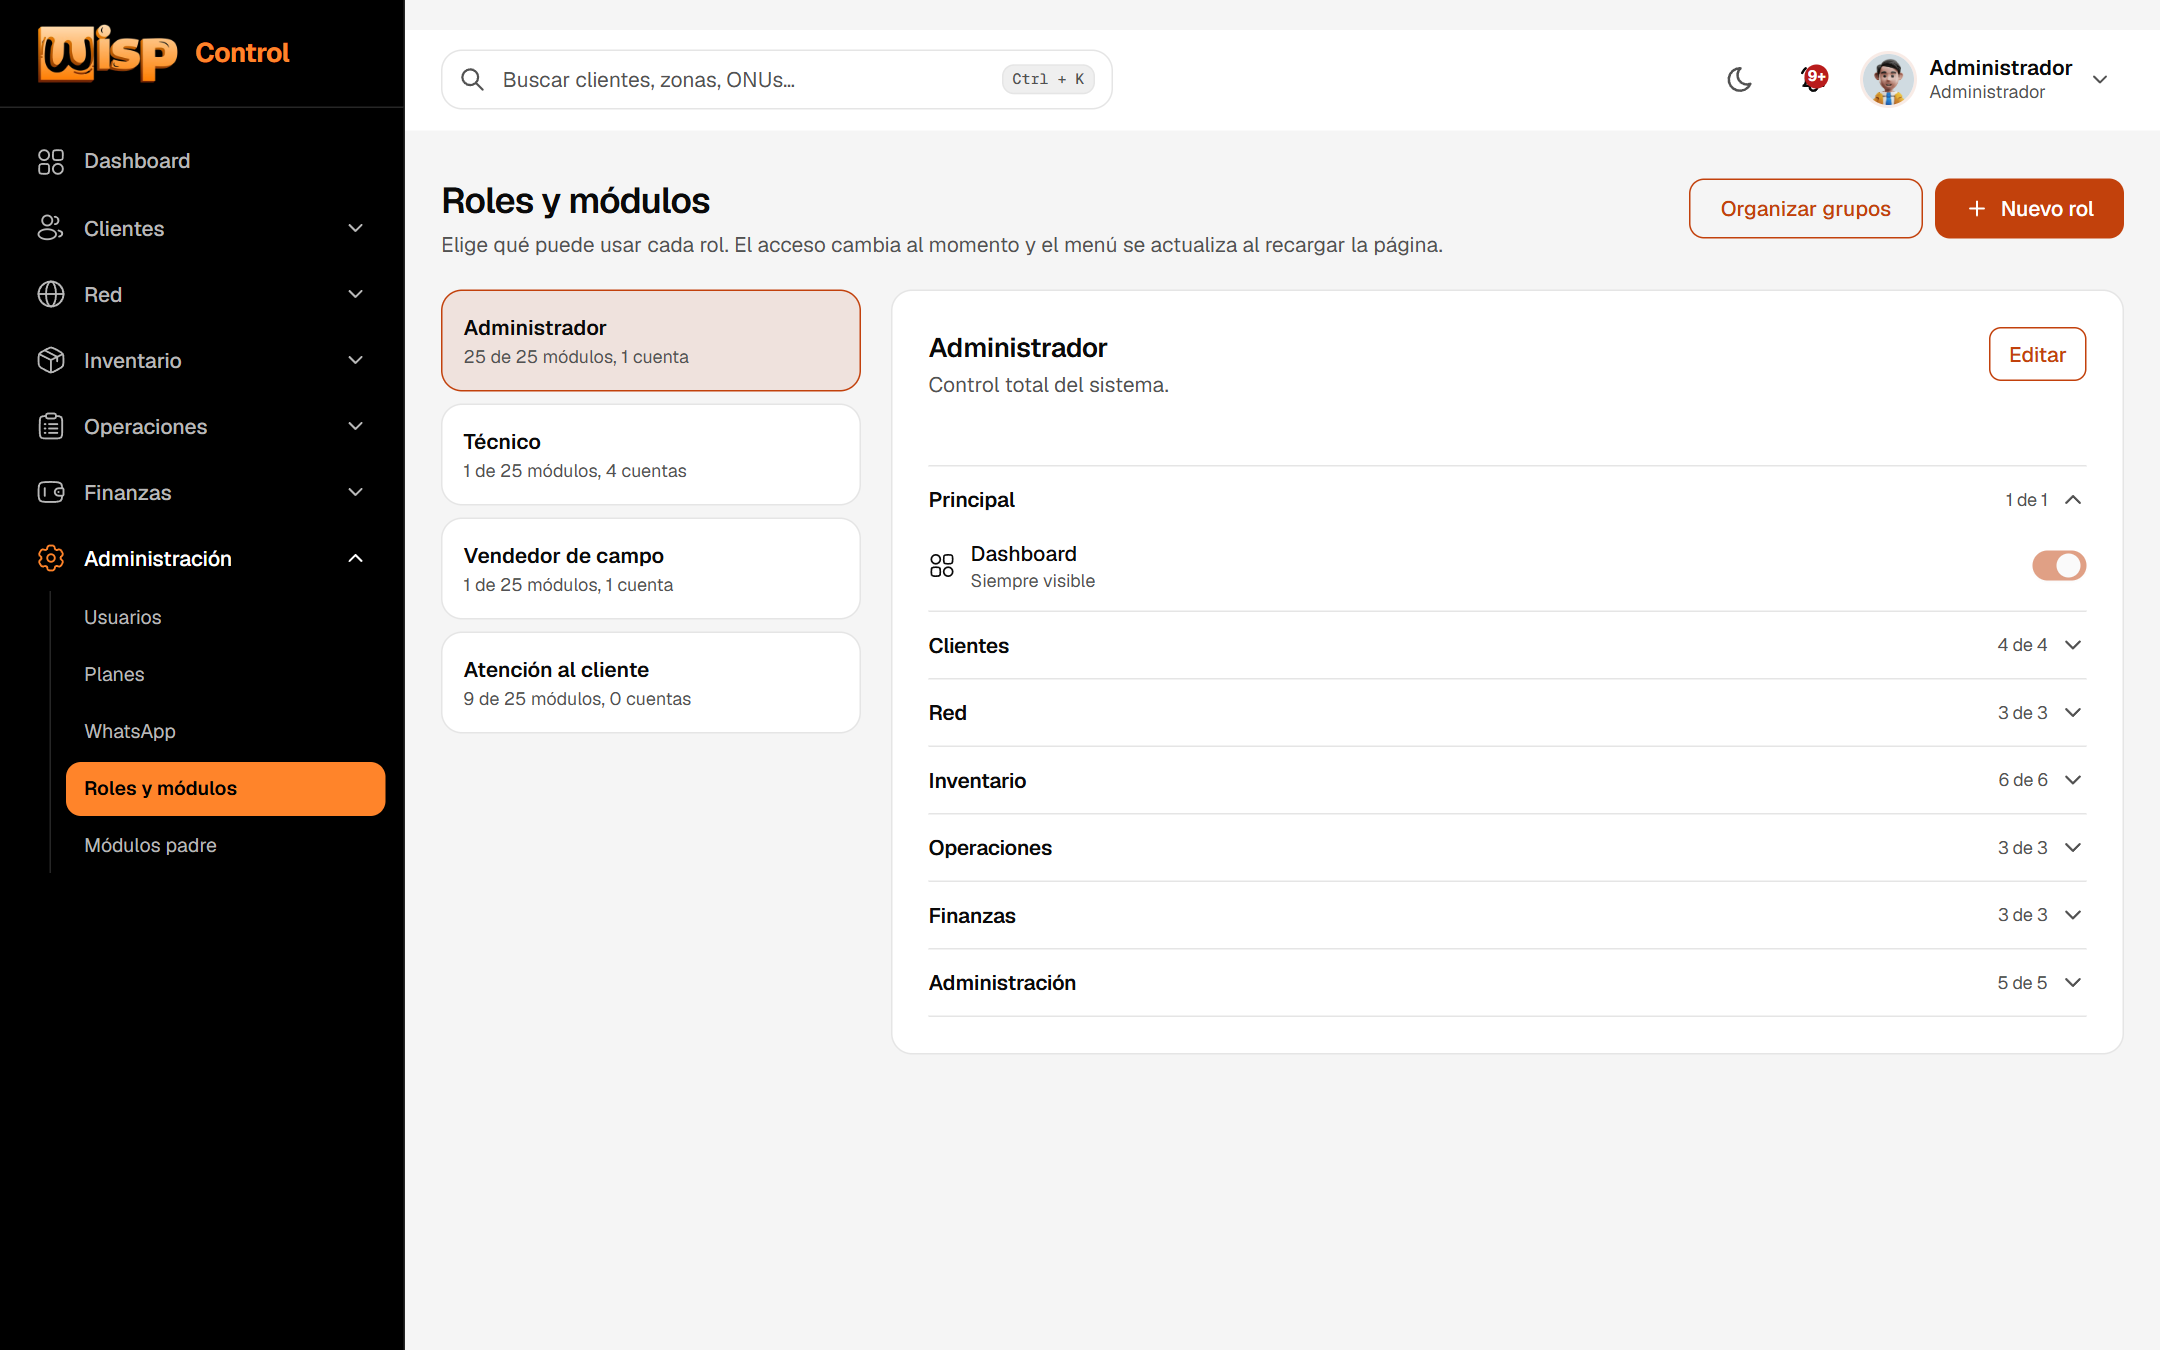
\includegraphics[width=\textwidth]{linea2/panel/p12_roles.png}
\caption{Roles y módulos: cada rol activa o desactiva módulos agrupados; el menú del usuario cambia sin desplegar.}
\label{fig:ce02-e3-roles}
\end{figure}


% ======================================================================
\section{Sección 3: Código y diseño técnico}
\label{sec:ce02-e3-codigo}

\subsection{Estructura del repositorio}

\begin{table}[H]
\centering
\caption{Estructura del repositorio \texttt{Wisp-ISP}.}
\label{tab:ce02-e3-repo}
\small
\begin{tabularx}{\textwidth}{L{4.4cm}X}
\toprule
\textbf{Carpeta} & \textbf{Contenido} \\
\midrule
\texttt{backend/app/} & \texttt{main.py} (arranque y CORS), \texttt{config.py} (variables de entorno), \texttt{models.py}, \texttt{schemas.py}, \texttt{acceso.py} (módulos por endpoint), \texttt{scheduler.py}, \texttt{recibos.py}, \texttt{facturacion.py} \\
\texttt{backend/app/routers/} & 19 routers, uno por dominio (clientes, zonas, pagos, permisos\ldots) \\
\texttt{backend/alembic/versions/} & 35 migraciones del esquema \\
\texttt{backend/tests/} & Pruebas con pytest y su configuración (\texttt{conftest.py}) \\
\texttt{frontend/src/} & Panel React: \texttt{views/} por módulo, \texttt{components/}, \texttt{lib/} (clientes de API por dominio) \\
\texttt{mobile/app/}, \texttt{mobile/src/} & App Expo: pantallas por rol y servicios (\texttt{services/api.ts}) \\
\texttt{whatsapp/} & Servicio de mensajería \\
\texttt{web/} & Sitio público estático \\
\texttt{nginx/} & Proxy inverso para servidor con IP pública o detrás de Cloudflare \\
\texttt{docs/}, \texttt{scripts/} & Guía de despliegue en la oficina y script de despliegue \\
\texttt{docker-compose*.yml} & Orquestación de los 7 servicios \\
\bottomrule
\end{tabularx}
\end{table}

\subsection{Patrones y buenas prácticas aplicadas}

\begin{itemize}
  \item \textbf{Modularidad por dominio:} cada router agrupa los endpoints de un dominio del
  negocio; el panel tiene una carpeta de vistas y un cliente de API por dominio.
  \item \textbf{Inyección de dependencias de FastAPI:} la sesión de base de datos
  (\texttt{get\_db}), el usuario actual y los roles se declaran como dependencias en la firma
  de cada endpoint, por lo que la seguridad es visible y no se puede olvidar en el cuerpo.
  \item \textbf{Esquemas de entrada y salida:} Pydantic valida cada petición y define qué
  campos salen en cada respuesta (por ejemplo, la red de una zona solo se entrega al
  administrador).
  \item \textbf{Adaptadores hacia sistemas externos:} el acceso a los routers, a la VPS, a
  WhatsApp y a APIs Perú está encapsulado en funciones propias; los endpoints no ejecutan
  comandos directamente.
  \item \textbf{Configuración externa:} todos los parámetros y secretos llegan por variables de
  entorno; el repositorio solo trae \texttt{.env.example} sin valores.
  \item \textbf{Esquema versionado:} cada cambio del modelo es una migración revisable.
  \item \textbf{Rendimiento consciente:} caché del estado WireGuard, consultas de resumen con
  \texttt{GROUP BY} en lugar de traer listas completas, y una sola sesión SSH por caja para ver
  el estado PPPoE de todos sus abonados.
\end{itemize}

\subsection{Manejo de errores y validaciones}

\begin{itemize}
  \item Las reglas de negocio devuelven errores HTTP con mensajes claros en español
  (\texttt{HTTPException}): por ejemplo, ``El cliente no está aprobado para instalación''.
  \item Las validaciones se hacen antes de tocar el router: la fecha de instalación no puede
  ser futura ni de hace más de una semana, porque de ella sale el día de pago.
  \item La base de datos rechaza duplicados críticos (número de operación de pago, número de
  borne por caja, DNI, usuario PPPoE).
  \item Las operaciones con routers informan si el equipo no respondió y no dejan el registro a
  medias (por ejemplo, el secreto PPPoE existente se vincula en vez de duplicarse).
  \item En producción el backend se niega a arrancar si las claves siguen con valores de
  ejemplo, y el inicio de sesión se bloquea tras 8 intentos fallidos en 5 minutos.
  \item Los borrados están restringidos: no se puede eliminar un usuario con actividad, una
  caja con bornes ocupados ni una zona con clientes.
\end{itemize}

\subsection{Desempeño y comportamiento en producción}
\label{sec:ce02-e3-desempeno}

Se midió el sistema en producción el 19/11/2026 con el script
\texttt{tools/medir\_desempeno.py}: 30 peticiones secuenciales a cada una de cinco rutas
públicas de \texttt{wispfibra.com}, desde un equipo del proyecto conectado por internet. Es
una carga deliberadamente ligera, para no afectar el servicio. Cada petición abre una
conexión nueva, por lo que el tiempo incluye la conexión TCP y la negociación TLS.

\begin{table}[H]
\centering
\caption{Tiempos de respuesta en producción (milisegundos; 30 peticiones por ruta).}
\label{tab:ce02-e3-desempeno}
\small
\begin{tabularx}{\textwidth}{XC{1.2cm}C{1.4cm}C{1.2cm}C{1.2cm}C{1.2cm}C{1.3cm}}
\toprule
\textbf{Ruta} & \textbf{Éxito} & \textbf{TTFB (mediana)} & \textbf{p50} & \textbf{p95} & \textbf{Máx.} & \textbf{Tamaño (KB)} \\
\midrule
\csname @@input\endcsname capitulos/linea2/tablas/desempeno.tex
\bottomrule
\end{tabularx}
\end{table}

\begin{table}[H]
\centering
\caption{Dónde se va el tiempo de una petición (medianas).}
\label{tab:ce02-e3-latencia}
\small
\begin{tabularx}{\textwidth}{L{5.4cm}C{2cm}X}
\toprule
\textbf{Tramo} & \textbf{Tiempo} & \textbf{Interpretación} \\
\midrule
Conexión TCP hasta Cloudflare & $\approx$ 120 ms & El nodo que atiende está en Río de Janeiro (\texttt{CF-RAY \ldots-GIG}). \\
Negociación TLS & $\approx$ 115 ms & Se paga una vez por conexión; el navegador y la app la reutilizan. \\
Cloudflare $\rightarrow$ túnel $\rightarrow$ servidor $\rightarrow$ regreso & $\approx$ 230 ms & Ida y vuelta Perú--Brasil--Perú hasta el servidor de la oficina. \\
Procesamiento de la API & 3--7 ms & Diferencia entre \texttt{/api/health} (sin trabajo) y las rutas que consultan la base. \\
Petición con la conexión ya abierta & $\approx$ 229 ms & Lo que percibe un usuario al navegar por el panel. \\
\bottomrule
\end{tabularx}
\end{table}

\paragraph{Lectura de los resultados.}
\begin{itemize}
  \item \textbf{Estabilidad:} 150 de 150 peticiones respondieron con éxito; la diferencia
  entre la mediana y el percentil 95 es de menos de 130 ms en todas las rutas.
  \item \textbf{El servidor no es el cuello de botella:} la API procesa en milisegundos; casi
  todo el tiempo es red. Coincide con lo medido en la base de datos, donde las consultas
  principales tardan menos de 1 ms con los índices propuestos (\cref{tab:ce02-indices}).
  \item \textbf{Mejora posible:} el sitio público se entrega sin caché de Cloudflare
  (\texttt{cf-cache-status: DYNAMIC}). Habilitar caché para los archivos estáticos (imágenes,
  CSS, JS) evitaría el viaje hasta la oficina en la mayoría de las visitas.
  \item \textbf{Comportamiento interno:} el sistema ya evita cargas innecesarias: guarda 120 s
  el estado de WireGuard en lugar de consultar la VPS en cada pantalla, cuenta los clientes
  por estado con una sola consulta \texttt{GROUP BY} y consulta el PPPoE de todos los abonados
  de una caja en una única sesión SSH. El servicio de WhatsApp tiene un techo de 0,5 CPU y
  512 MB para que una falla suya no tumbe el servidor.
\end{itemize}

\subsection{Escalabilidad y diseño técnico}
\label{sec:ce02-e3-escalabilidad}

\begin{table}[H]
\centering
\caption{Capacidad actual y cómo crece cada dimensión.}
\label{tab:ce02-e3-escala}
\small
\begin{tabularx}{\textwidth}{L{2.8cm}L{4cm}X}
\toprule
\textbf{Dimensión} & \textbf{Hoy} & \textbf{Cómo crece} \\
\midrule
Zonas & 13 zonas & Una zona nueva es un registro, un peer WireGuard y la sincronización de planes desde el panel; no requiere cambiar código. \\
Clientes & Unos 455 & El modelo y los índices soportan decenas de miles (probado con 50\,000 clientes y 600\,000 pagos, \cref{sec:ce02-optimizacion}). \\
Personal y permisos & 4 tipos de cuenta, roles configurables & Se crean roles y se asignan módulos desde el panel, sin desplegar. \\
Tráfico web & Publicación por Cloudflare & Cloudflare absorbe el TLS y el tráfico malicioso; el servidor solo recibe peticiones válidas. \\
Servidor & Un equipo de escritorio (4 núcleos, 4 GB), 1,3--1,8 GB de RAM en reposo & Es el límite real: se reemplaza por el servidor definitivo o se migra al diseño híbrido del semestre~1 (\cref{chap:ce03-dc}) con el mismo Docker Compose. \\
\bottomrule
\end{tabularx}
\end{table}

\noindent \textbf{Límite para escalar horizontalmente.} El backend no guarda sesiones (usa
JWT), pero mantiene tres estados en la memoria del proceso: el freno de intentos de login
(\texttt{\_intentos} en \texttt{auth.py}), la caché del estado WireGuard y el planificador
APScheduler. Si se levantaran dos copias del backend, el freno de login se repartiría entre
ellas y los cortes de las 09:00 se ejecutarían dos veces. Para crecer a varias réplicas habría
que mover esos estados a un almacén compartido (por ejemplo, Redis) y dejar el planificador
en una sola instancia. Con el volumen actual de WISP no es necesario: una sola instancia
atiende la carga con holgura.

% ======================================================================
\section{Sección 4: Despliegue o instalación}
\label{sec:ce02-e3-despliegue}

\begin{table}[H]
\centering
\caption{Servicios del despliegue con Docker Compose.}
\label{tab:ce02-e3-servicios}
\small
\begin{tabularx}{\textwidth}{L{3.2cm}L{3.4cm}X}
\toprule
\textbf{Contenedor} & \textbf{Imagen / puerto} & \textbf{Notas} \\
\midrule
\texttt{wisp\_postgres} & PostgreSQL 15, 127.0.0.1:5432 & Volumen \texttt{postgres\_data}; chequeo de salud. \\
\texttt{wisp\_backend} & FastAPI, 8000 (red del host) & Aplica migraciones al arrancar; monta respaldos, evidencias, llaves SSH. \\
\texttt{wisp\_frontend} & Panel compilado, 127.0.0.1:3000 & Servido con Nginx. \\
\texttt{wisp\_web} & Sitio estático, 127.0.0.1:3002 & --- \\
\texttt{wisp\_whatsapp} & Node + Baileys, 127.0.0.1:3001 & Límite de 0,5 CPU y 512 MB; sesión en volumen. \\
\texttt{wisp\_nginx} & Nginx, 80 & Enruta \texttt{/}, \texttt{/app} y \texttt{/api}; cabeceras de seguridad. \\
\texttt{wisp\_cloudflared} & Cloudflare Tunnel & Publica \texttt{wispfibra.com} sin puertos de entrada. \\
\bottomrule
\end{tabularx}
\end{table}

\paragraph{Configuración requerida.} El archivo \texttt{.env} (a partir de
\texttt{.env.example}) define: base de datos, clave del JWT y vigencia de la sesión (8~h),
orígenes CORS, freno a la fuerza bruta, administrador inicial, URL y token del servicio de
WhatsApp, datos de la VPS y del túnel WireGuard, rutas de respaldos y evidencias, días de
gracia, datos de la empresa para el recibo, archivo de Nginx a usar, token del túnel de
Cloudflare y token de APIs Perú.

\paragraph{Instalación.}
\begin{lstlisting}[style=plano]
git clone https://github.com/cristian-csc/Wisp-ISP.git && cd Wisp-ISP
cp .env.example .env && chmod 600 .env          # completar los valores reales
# en .env: NGINX_CONF=nginx.cloudflare.conf y CLOUDFLARE_TUNNEL_TOKEN=<token>
docker compose -f docker-compose.yml -f docker-compose.cloudflare.yml up -d --build
docker compose ps                                # todos los contenedores en "running"
\end{lstlisting}

\paragraph{App móvil.} Se compila con EAS (\texttt{eas build}) usando
\texttt{EXPO\_PUBLIC\_API\_URL=https://wispfibra.com/api}. La evidencia del despliegue es la
verificación de la \cref{tab:ce02-e3-verificacion} y las capturas del sitio y del panel en
producción.

% ======================================================================
\section{Anexos del entregable}
\label{sec:ce02-e3-anexos}

\subsection{Catálogo completo de la API}

Se genera automáticamente desde el código con los scripts \texttt{extraer\_endpoints.py} y
\texttt{catalogo\_api.py} de la carpeta \texttt{tools}. La columna \emph{Acceso} indica el tipo de cuenta exigido; en
los endpoints marcados como ``autenticado'' y en muchos de los demás, \texttt{acceso.py}
exige además que el rol tenga el módulo correspondiente.

{\footnotesize
\begin{longtable}{L{1.0cm}L{5.3cm}L{2.3cm}L{5.6cm}}
\caption{Endpoints de la API REST (169).}\label{tab:ce02-e3-catalogo}\\
\toprule
\textbf{Método} & \textbf{Ruta} & \textbf{Acceso} & \textbf{Descripción} \\
\midrule
\endfirsthead
\toprule
\textbf{Método} & \textbf{Ruta} & \textbf{Acceso} & \textbf{Descripción} \\
\midrule
\endhead
\bottomrule
\endlastfoot
\csname @@input\endcsname capitulos/linea2/tablas/catalogo_api.tex
\end{longtable}
}

\subsection{Manual técnico breve}
\label{sec:ce02-e3-manual}

Dirigido a quien administre el sistema. Supone un servidor con Ubuntu Server 24.04, Docker y
el repositorio clonado en \texttt{\textasciitilde/Wisp-ISP}. No incluye contraseñas ni llaves:
se guardan fuera del repositorio.

\paragraph{1. Instalación inicial.} Ver la \cref{sec:ce02-e3-despliegue}. Antes de instalar:
encendido automático tras corte de energía en la BIOS, UPS, revisión del disco
(\texttt{smartctl -H}) y 4~GB de memoria de intercambio si el equipo tiene 4~GB de RAM.

\paragraph{2. Actualizar a una versión nueva.}
\begin{lstlisting}[style=plano]
cd ~/Wisp-ISP && git pull
docker compose -f docker-compose.yml -f docker-compose.cloudflare.yml up -d --build
docker compose logs --tail=50 backend      # las migraciones se aplican solas al arrancar
\end{lstlisting}

\paragraph{3. Respaldo y restauración de la base de datos.}
\begin{lstlisting}[style=plano]
# respaldo manual (el diario se programa con cron a las 03:00)
docker exec wisp_postgres pg_dump -U <USUARIO> <BASE> | gzip > db_$(date +%F).sql.gz
# restauración en un servidor nuevo
docker compose up -d postgres
gunzip -c db_AAAA-MM-DD.sql.gz | docker exec -i wisp_postgres psql -U <USUARIO> <BASE>
\end{lstlisting}
Las evidencias fotográficas se respaldan aparte (\texttt{/opt/wisp-isp/media}). Ambas copias
deben salir del servidor (ver el plan de continuidad del SGSI).

\paragraph{4. Agregar una zona nueva.} (1) Crear la zona en el panel (Red $\rightarrow$
Zonas) con su pool PPPoE y el nombre exacto de su lista de corte. (2) Generar las llaves
WireGuard en el MikroTik y registrar su llave pública en la ficha de la zona. (3) Configurar
en el router el peer del hub con los datos que devuelve el panel. (4) Verificar el estado del
túnel en la ficha. (5) Ejecutar la verificación de planes para comparar los perfiles PPPoE del
router con los del panel. (6) Asignar los técnicos de la zona.

\paragraph{5. Dar de alta a un colaborador.} Administración $\rightarrow$ Usuarios: crear la
cuenta con su tipo de cuenta y rol; si es técnico, asignarle sus zonas. Los módulos que verá se
ajustan en Administración $\rightarrow$ Roles y módulos. Al cese, desactivar la cuenta (no
borrarla si tuvo actividad).

\paragraph{6. Solución de problemas frecuentes.} La \cref{tab:ce02-e3-problemas} reúne los
síntomas más comunes y qué revisar primero en cada caso.

\begin{table}[H]
\centering
\caption{Problemas frecuentes y cómo resolverlos.}
\label{tab:ce02-e3-problemas}
\small
\begin{tabularx}{\textwidth}{L{4cm}X}
\toprule
\textbf{Síntoma} & \textbf{Qué revisar} \\
\midrule
El sitio no carga & \texttt{docker compose ps}; registro de \texttt{wisp\_cloudflared} (debe decir ``Registered tunnel connection''); token del túnel en el \texttt{.env}. \\
El panel carga, pero da error al entrar & Estado de \texttt{wisp\_backend} y su registro; el firewall del servidor no debe cerrar el puerto 8000 a la red de Docker. \\
No llegan los WhatsApp & Estado de la sesión en Administración $\rightarrow$ WhatsApp; si se desvinculó, escanear el QR de nuevo; \texttt{docker stats wisp\_whatsapp} (techo de 512 MB). \\
Una zona aparece fuera de línea & Estado WireGuard de la zona; energía y enlace del router; último \emph{handshake} en la VPS. \\
Un corte no corta & El nombre de la lista de corte de la zona debe coincidir exactamente con el del router (por ejemplo, \texttt{CORTE MOROSO}). \\
El servidor va lento & \texttt{free -h} (uso de memoria de intercambio) y \texttt{df -h} (las evidencias llenan el disco). \\
\bottomrule
\end{tabularx}
\end{table}

\subsection{Diagramas editables}

Los diagramas de este capítulo están escritos en Mermaid en la carpeta
\texttt{diagramas/ce02\_e3/}. Se pueden importar en Lucidchart o en draw.io para editarlos,
y regenerar las imágenes del documento desde el mismo archivo.

\begin{table}[H]
\centering
\caption{Fuentes de los diagramas.}
\label{tab:ce02-e3-diagramas}
\small
\begin{tabularx}{\textwidth}{L{5.4cm}X}
\toprule
\texttt{d01\_mapa\_negocio.mmd} & Mapa del giro del negocio (\cref{fig:ce02-e3-mapa}) \\
\texttt{d02\_venta\_instalacion.mmd} & Captación, aprobación e instalación (\cref{fig:ce02-e3-venta}) \\
\texttt{d03\_cobranza\_corte.mmd} & Cobranza, corte y reactivación (\cref{fig:ce02-e3-cobranza}) \\
\texttt{d04\_averias\_retiros.mmd} & Averías y retiros (\cref{fig:ce02-e3-averias}) \\
\texttt{d05\_jornada\_vendedor.mmd} & Jornada del vendedor (\cref{fig:ce02-e3-jornada}) \\
\texttt{d06\_roles\_modulos.mmd} & Modelo de permisos (\cref{fig:ce02-e3-permisos}) \\
\texttt{d07\_app\_movil.mmd} & Navegación de la app móvil (\cref{fig:ce02-e3-movil}) \\
\texttt{d08\_panel\_web.mmd} & Mapa del panel web (\cref{fig:ce02-e3-panel}) \\
\texttt{d09\_alta\_zona\_wireguard.mmd} & Alta de zona y túnel WireGuard (\cref{fig:ce02-e3-zona-wg}) \\
\bottomrule
\end{tabularx}
\end{table}

\noindent Pendiente: la evidencia de sustentación (demo ante el docente).
